\documentclass[ignorenonframetext,a4paper]{beamer}
\setbeamertemplate{caption}[numbered]
\setbeamertemplate{caption label separator}{: }
\setbeamercolor{caption name}{fg=normal text.fg}
\beamertemplatenavigationsymbolsempty
\usepackage{lmodern}
\usepackage{amssymb,amsmath}
\usepackage{ifxetex,ifluatex}
\usepackage{fixltx2e} % provides \textsubscript
\ifnum 0\ifxetex 1\fi\ifluatex 1\fi=0 % if pdftex
  \usepackage[T1]{fontenc}
  \usepackage[utf8]{inputenc}
\else % if luatex or xelatex
  \ifxetex
    \usepackage{mathspec}
  \else
    \usepackage{fontspec}
  \fi
  \defaultfontfeatures{Ligatures=TeX,Scale=MatchLowercase}
\fi
\usetheme[]{Padova}
% use upquote if available, for straight quotes in verbatim environments
\IfFileExists{upquote.sty}{\usepackage{upquote}}{}
% use microtype if available
\IfFileExists{microtype.sty}{%
\usepackage{microtype}
\UseMicrotypeSet[protrusion]{basicmath} % disable protrusion for tt fonts
}{}
\newif\ifbibliography
\hypersetup{
            pdfborder={0 0 0},
            breaklinks=true}
\urlstyle{same}  % don't use monospace font for urls
\usepackage{color}
\usepackage{fancyvrb}
\newcommand{\VerbBar}{|}
\newcommand{\VERB}{\Verb[commandchars=\\\{\}]}
\DefineVerbatimEnvironment{Highlighting}{Verbatim}{commandchars=\\\{\}}
% Add ',fontsize=\small' for more characters per line
\usepackage{framed}
\definecolor{shadecolor}{RGB}{248,248,248}
\newenvironment{Shaded}{\begin{snugshade}}{\end{snugshade}}
\newcommand{\KeywordTok}[1]{\textcolor[rgb]{0.13,0.29,0.53}{\textbf{#1}}}
\newcommand{\DataTypeTok}[1]{\textcolor[rgb]{0.13,0.29,0.53}{#1}}
\newcommand{\DecValTok}[1]{\textcolor[rgb]{0.00,0.00,0.81}{#1}}
\newcommand{\BaseNTok}[1]{\textcolor[rgb]{0.00,0.00,0.81}{#1}}
\newcommand{\FloatTok}[1]{\textcolor[rgb]{0.00,0.00,0.81}{#1}}
\newcommand{\ConstantTok}[1]{\textcolor[rgb]{0.00,0.00,0.00}{#1}}
\newcommand{\CharTok}[1]{\textcolor[rgb]{0.31,0.60,0.02}{#1}}
\newcommand{\SpecialCharTok}[1]{\textcolor[rgb]{0.00,0.00,0.00}{#1}}
\newcommand{\StringTok}[1]{\textcolor[rgb]{0.31,0.60,0.02}{#1}}
\newcommand{\VerbatimStringTok}[1]{\textcolor[rgb]{0.31,0.60,0.02}{#1}}
\newcommand{\SpecialStringTok}[1]{\textcolor[rgb]{0.31,0.60,0.02}{#1}}
\newcommand{\ImportTok}[1]{#1}
\newcommand{\CommentTok}[1]{\textcolor[rgb]{0.56,0.35,0.01}{\textit{#1}}}
\newcommand{\DocumentationTok}[1]{\textcolor[rgb]{0.56,0.35,0.01}{\textbf{\textit{#1}}}}
\newcommand{\AnnotationTok}[1]{\textcolor[rgb]{0.56,0.35,0.01}{\textbf{\textit{#1}}}}
\newcommand{\CommentVarTok}[1]{\textcolor[rgb]{0.56,0.35,0.01}{\textbf{\textit{#1}}}}
\newcommand{\OtherTok}[1]{\textcolor[rgb]{0.56,0.35,0.01}{#1}}
\newcommand{\FunctionTok}[1]{\textcolor[rgb]{0.00,0.00,0.00}{#1}}
\newcommand{\VariableTok}[1]{\textcolor[rgb]{0.00,0.00,0.00}{#1}}
\newcommand{\ControlFlowTok}[1]{\textcolor[rgb]{0.13,0.29,0.53}{\textbf{#1}}}
\newcommand{\OperatorTok}[1]{\textcolor[rgb]{0.81,0.36,0.00}{\textbf{#1}}}
\newcommand{\BuiltInTok}[1]{#1}
\newcommand{\ExtensionTok}[1]{#1}
\newcommand{\PreprocessorTok}[1]{\textcolor[rgb]{0.56,0.35,0.01}{\textit{#1}}}
\newcommand{\AttributeTok}[1]{\textcolor[rgb]{0.77,0.63,0.00}{#1}}
\newcommand{\RegionMarkerTok}[1]{#1}
\newcommand{\InformationTok}[1]{\textcolor[rgb]{0.56,0.35,0.01}{\textbf{\textit{#1}}}}
\newcommand{\WarningTok}[1]{\textcolor[rgb]{0.56,0.35,0.01}{\textbf{\textit{#1}}}}
\newcommand{\AlertTok}[1]{\textcolor[rgb]{0.94,0.16,0.16}{#1}}
\newcommand{\ErrorTok}[1]{\textcolor[rgb]{0.64,0.00,0.00}{\textbf{#1}}}
\newcommand{\NormalTok}[1]{#1}
\usepackage{longtable,booktabs}
\usepackage{caption}
% These lines are needed to make table captions work with longtable:
\makeatletter
\def\fnum@table{\tablename~\thetable}
\makeatother
\usepackage{graphicx,grffile}
\makeatletter
\def\maxwidth{\ifdim\Gin@nat@width>\linewidth\linewidth\else\Gin@nat@width\fi}
\def\maxheight{\ifdim\Gin@nat@height>\textheight0.8\textheight\else\Gin@nat@height\fi}
\makeatother
% Scale images if necessary, so that they will not overflow the page
% margins by default, and it is still possible to overwrite the defaults
% using explicit options in \includegraphics[width, height, ...]{}
\setkeys{Gin}{width=\maxwidth,height=\maxheight,keepaspectratio}

% Prevent slide breaks in the middle of a paragraph:
\widowpenalties 1 10000
\raggedbottom

\AtBeginPart{
  \let\insertpartnumber\relax
  \let\partname\relax
  \frame{\partpage}
}
\AtBeginSection{
  \ifbibliography
  \else
    \let\insertsectionnumber\relax
    \let\sectionname\relax
    \frame{\sectionpage}
  \fi
}
\AtBeginSubsection{
  \let\insertsubsectionnumber\relax
  \let\subsectionname\relax
  \frame{\subsectionpage}
}

\setlength{\parindent}{0pt}
\setlength{\parskip}{6pt plus 2pt minus 1pt}
\setlength{\emergencystretch}{3em}  % prevent overfull lines
\providecommand{\tightlist}{%
  \setlength{\itemsep}{0pt}\setlength{\parskip}{0pt}}
\setcounter{secnumdepth}{0}
\usepackage{booktabs}
\usepackage{subfig}
\usepackage{multicol}
\usepackage{rotating}
\usepackage{mathtools}
\usepackage{pgfplots}
\usepackage{listings}
\usepackage{multirow}
\usepackage{amssymb}
\usepackage{pifont}
\usepackage{tikz}
\usepackage{graphics}
\usepackage{hyperref}
\usepackage{enumerate}
\hypersetup{ colorlinks = true, linkcolor = blue, filecolor = magenta, urlcolor = cyan,}

\title{\Large\textbf{Introduction to Bayesian Computation and Application to Regression Models and Survival Analysis}}
\subtitle{\large\textbf{\textrm{IBIG 2018}}}
\author{\centering\underline{\textbf{Daniele Bottigliengo}}\thanks{\tiny Unit of Biostatistics, Epidemiology and Public Health, Department of \newline Cardiac, Thoracic, Vascular Sciences and Public Health, University of Padua, Italy}}
\date{\centering\emph{Padova, Italy, November 22, 2018}}

\begin{document}
\frame{\titlepage}

\section{Survival Analysis Case
Study}\label{survival-analysis-case-study}

\begin{frame}{Survival Ovarian Cancer}

\begin{itemize}
\item
  Randomized trial comparing treatment of patients with advanced ovarian
  carcinoma (stages \(IIIB\) and \(IV\)) (Edmonson et al. 1979)
\item
  Two groups of patients:

  \begin{itemize}
  \item{Cyclophosphamide alone ($1 \> g/m^{2}$)}
  \item{Cyclophosphamide ($500 \> \mu g/m^{2}$) plus Adriamycin 
      ($40 \> \mu g/m2$)}
    \end{itemize}
\item
  Intravenous (IV) injection every \(3\) weeks
\end{itemize}

\end{frame}

\begin{frame}{The dataset (1)}

\begin{itemize}
\setlength\itemsep{1em}
  \item{$26$ women enrolled}
  \item{The following information were retrieved:}
  \begin{itemize}
    \item{Age}
    \item{Presence of residual disease}
    \item{ECOG performance}
  \end{itemize}
\item{Median follow-up time in the Cyclophosphamide group: 
      $448$ days}
\item{Median follow-up time in the Cyclophosphamide plus 
      Adriamycin: $563$ days}  
\item{$12$ patients died during the study and $14$ were right-censored}
\end{itemize}

\end{frame}

\begin{frame}{The dataset (2)}

\tiny

\begin{longtable}[]{@{}rlrllr@{}}
\toprule
follow\_up\_days & status & age & residual\_disease & treatment &
ecog\_performance\tabularnewline
\midrule
\endhead
59 & dead & 72.3315 & yes & Cyclo & 1\tabularnewline
115 & dead & 74.4932 & yes & Cyclo & 1\tabularnewline
156 & dead & 66.4658 & yes & Cyclo & 2\tabularnewline
421 & alive & 53.3644 & yes & Cyclo + Adria & 1\tabularnewline
431 & dead & 50.3397 & yes & Cyclo & 1\tabularnewline
448 & alive & 56.4301 & no & Cyclo & 2\tabularnewline
464 & dead & 56.9370 & yes & Cyclo + Adria & 2\tabularnewline
475 & dead & 59.8548 & yes & Cyclo + Adria & 2\tabularnewline
477 & alive & 64.1753 & yes & Cyclo & 1\tabularnewline
563 & dead & 55.1781 & no & Cyclo + Adria & 2\tabularnewline
\bottomrule
\end{longtable}

\end{frame}

\begin{frame}{Exploratory data analysis (1)}

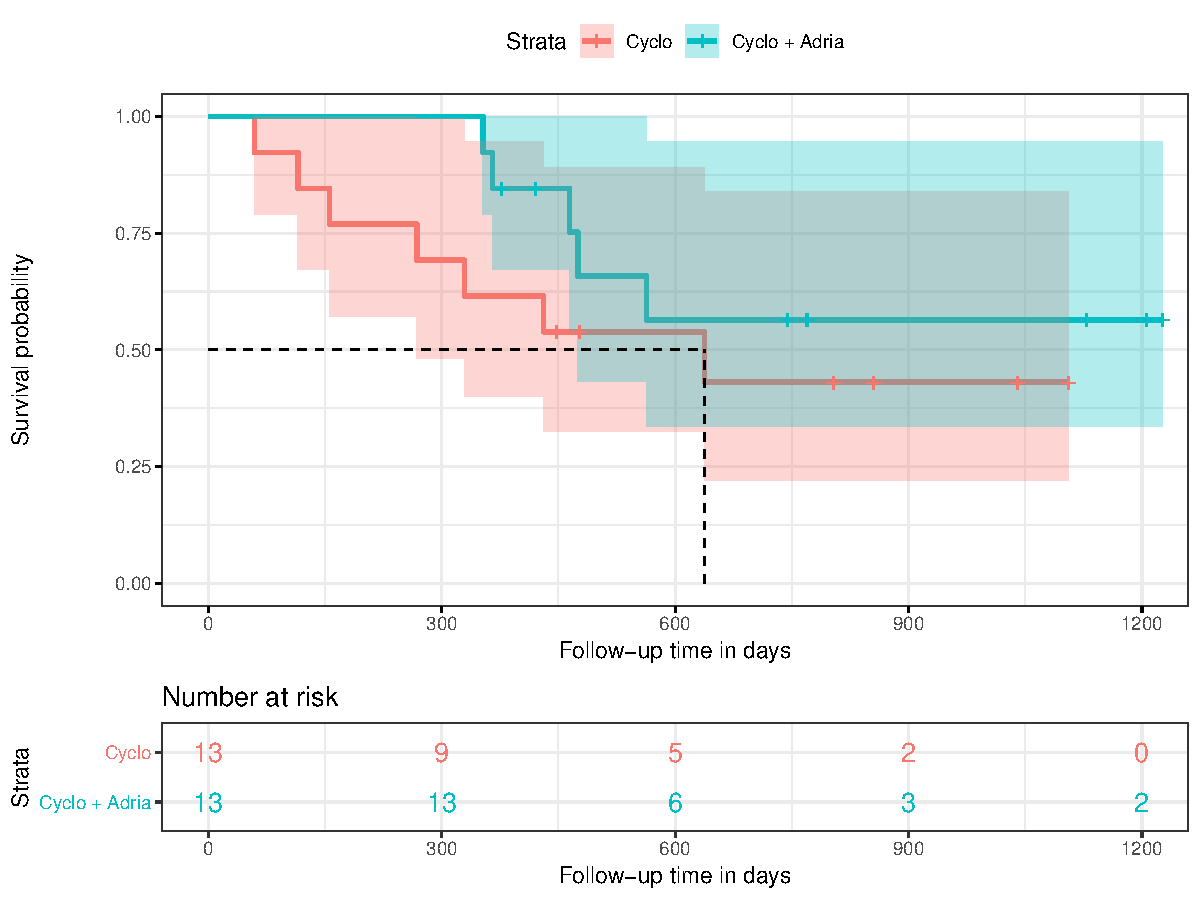
\includegraphics{DB_presentation_case_study_files/figure-beamer/unnamed-chunk-3-1.pdf}

\end{frame}

\begin{frame}{Exploratory data analysis (2)}

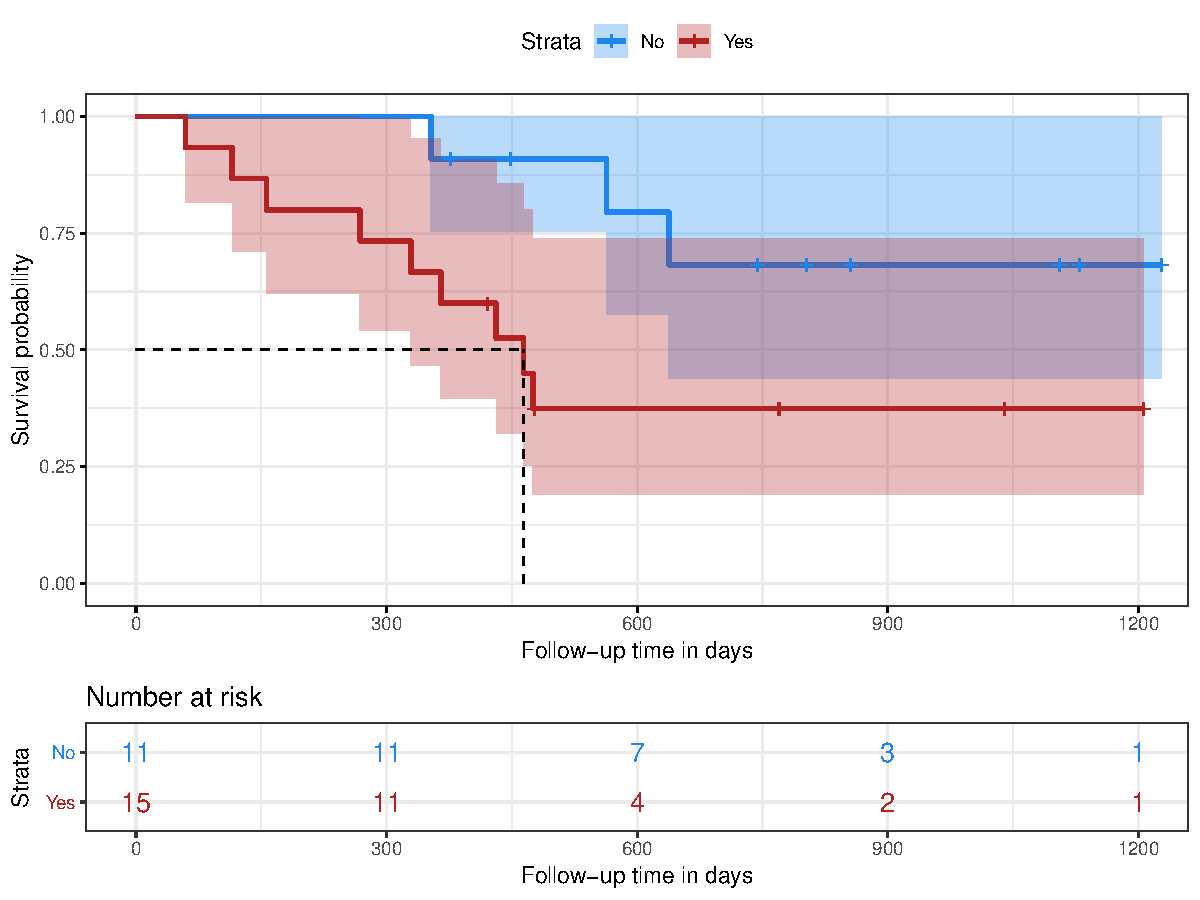
\includegraphics{DB_presentation_case_study_files/figure-beamer/unnamed-chunk-4-1.pdf}

\end{frame}

\begin{frame}{Exploratory data analysis (3)}

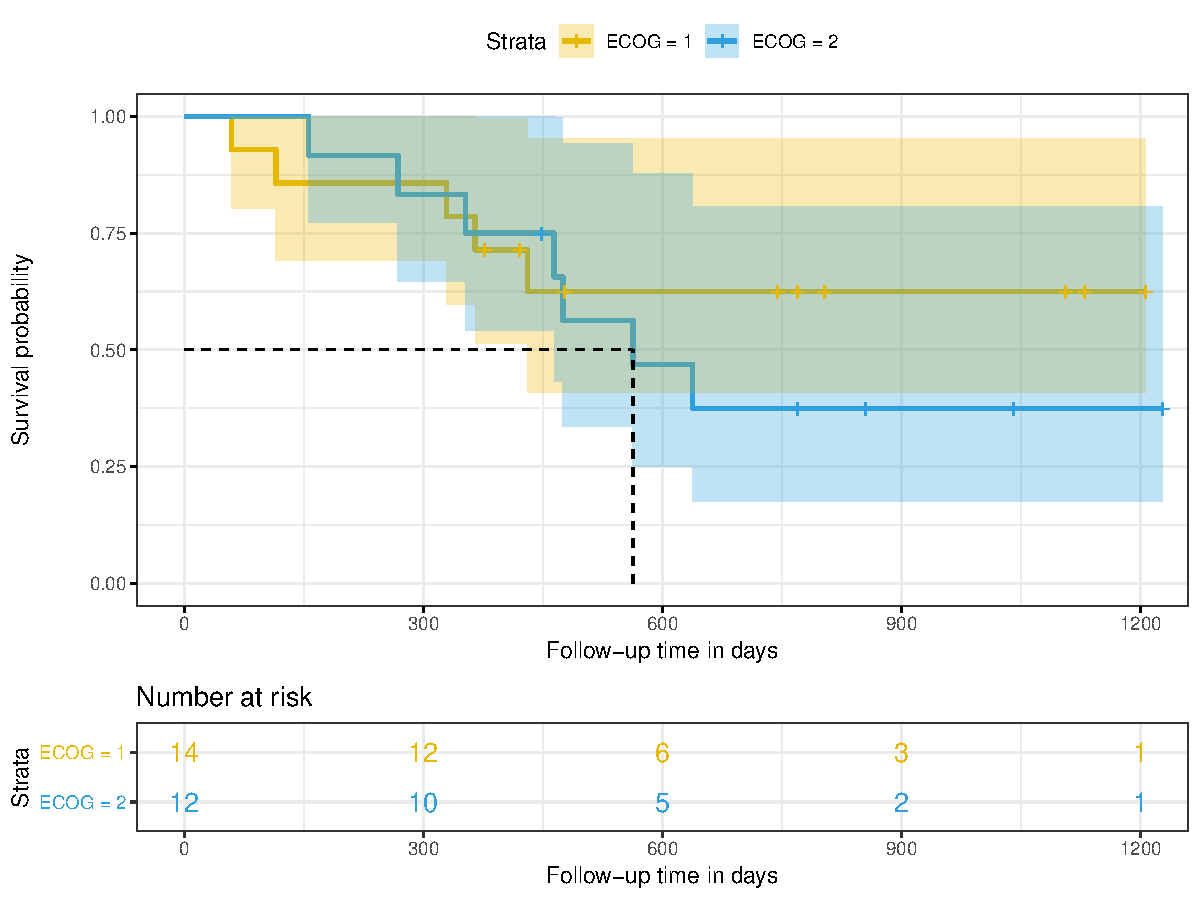
\includegraphics{DB_presentation_case_study_files/figure-beamer/unnamed-chunk-5-1.pdf}

\end{frame}

\begin{frame}{Survival Model}

Weibull parametric proportional hazard model: \[
  f \left( t \vert \alpha, \sigma \right) = \frac{\alpha}{\sigma} \left( \frac{t}{\sigma}\right)^{\alpha - 1} e ^{ - \left( \frac{t}{\sigma} \right)^{\alpha} }
  \] where:

\begin{itemize}
 \item{$\alpha$ is the shape parameter}
 \item{$\sigma$ is the scale parameter defined as $\sigma = e ^{ - \left( \frac{\eta}{\alpha} \right) }$}.
 \item{$\eta$ is the linear predictor and it can be expressed as 
       function of some covariates}
\end{itemize}

\end{frame}

\begin{frame}{Data simulations}

How to proceed:

\begin{enumerate}
  \item{Draw a parameter value from the prior distributions}
  \item{Simulate data according to the model and the parameters 
        values drawn from the priors}
  \item{Are simulated plausible?}
  \item{Fit the model to the simulated data}
  \item{Are true parameters values included in the posterior 
        distributions?}
\end{enumerate}

\end{frame}

\begin{frame}{Inspect simulated data}

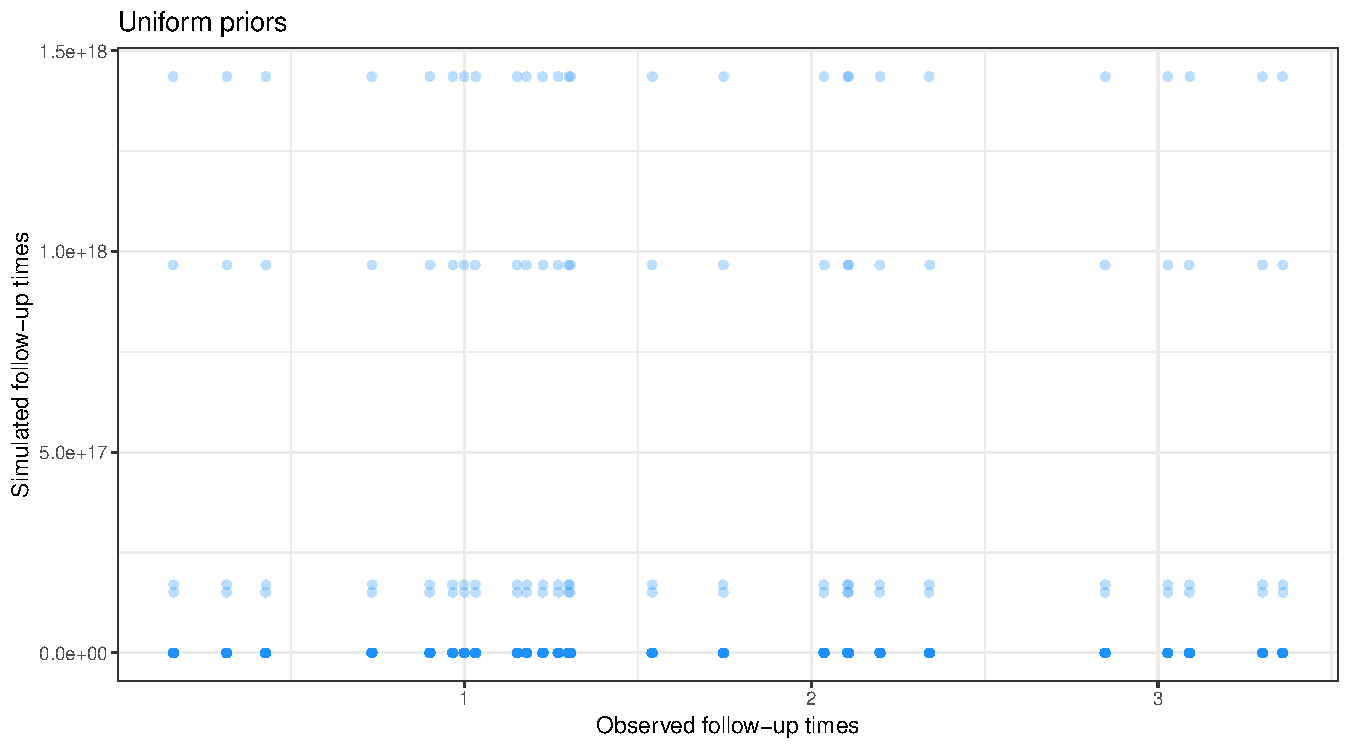
\includegraphics{DB_presentation_case_study_files/figure-beamer/unnamed-chunk-6-1.pdf}

\end{frame}

\begin{frame}{Inspect simulated data}

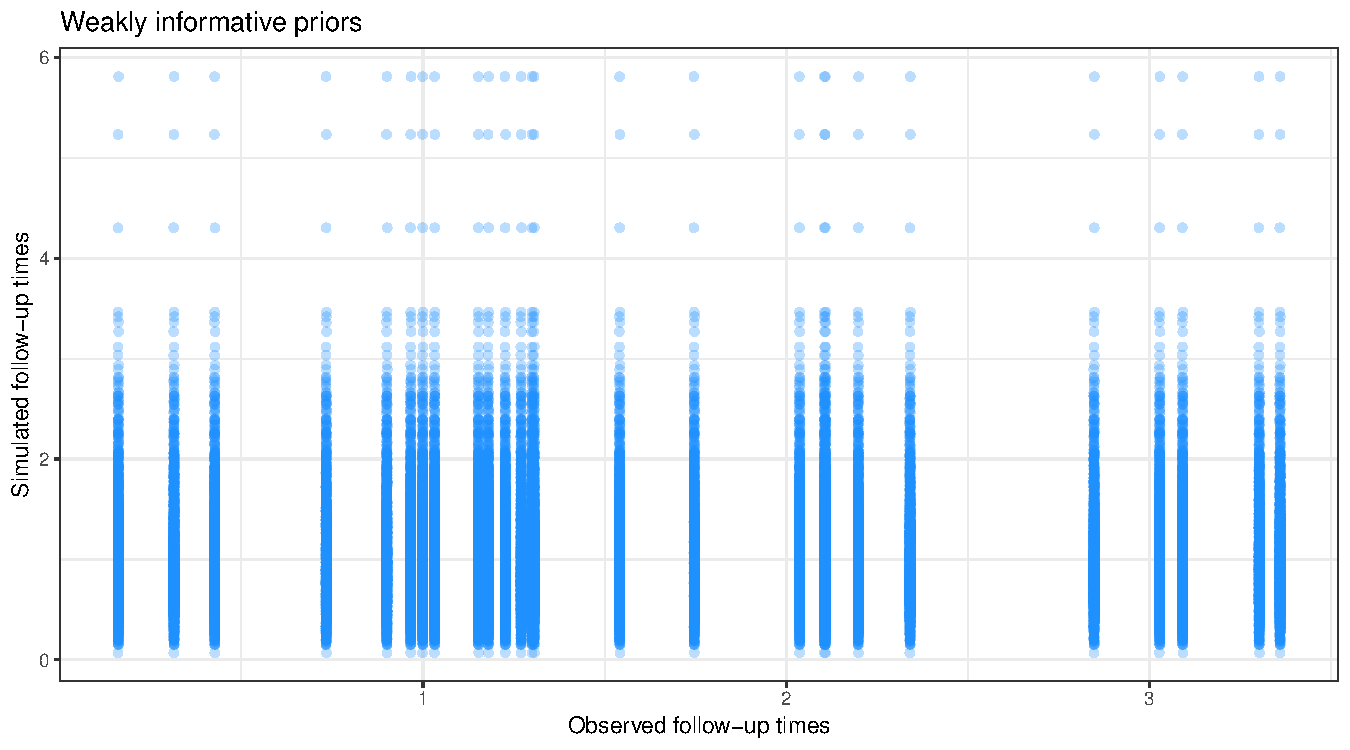
\includegraphics{DB_presentation_case_study_files/figure-beamer/unnamed-chunk-7-1.pdf}

\end{frame}

\begin{frame}{Recover the parameters values}

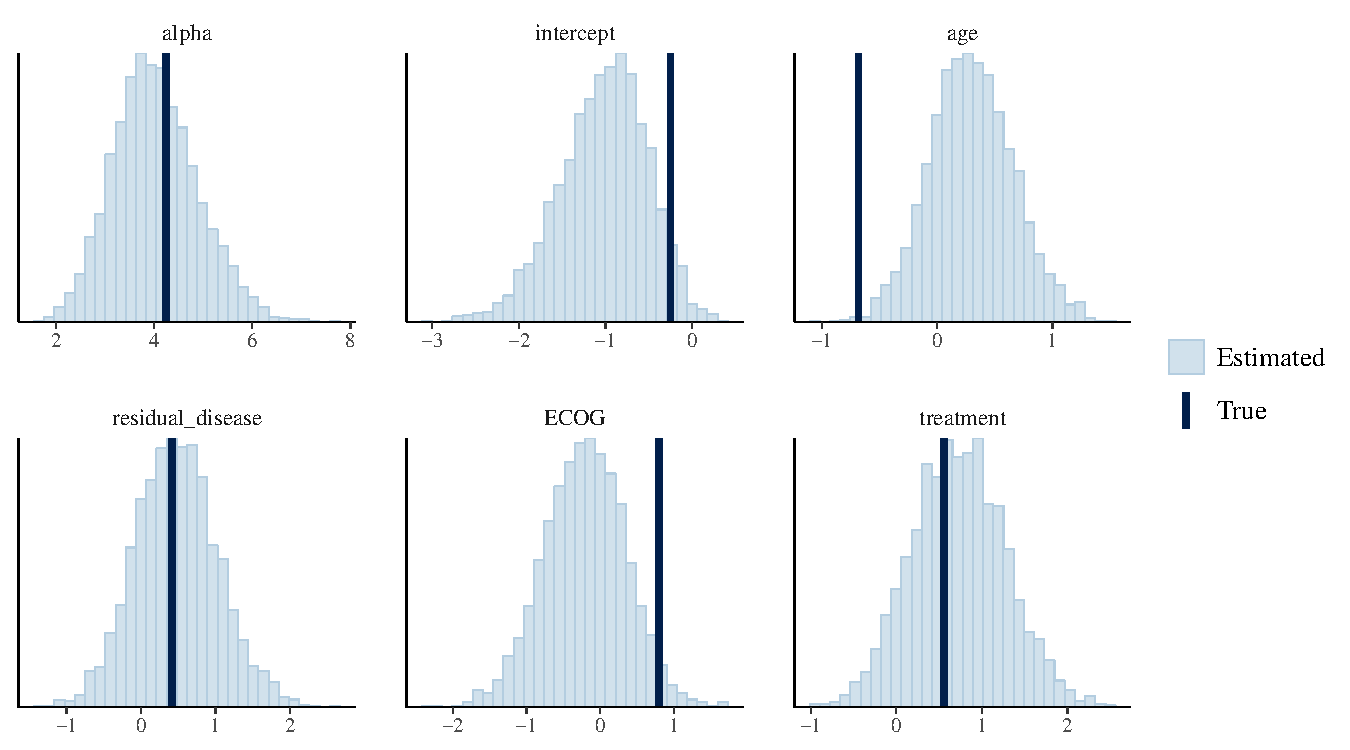
\includegraphics{DB_presentation_case_study_files/figure-beamer/unnamed-chunk-8-1.pdf}

\end{frame}

\begin{frame}[fragile]{The model: data block}

\scriptsize

\begin{Shaded}
\begin{Highlighting}[]
\StringTok{"}
\StringTok{data \{}

\StringTok{  int<lower = 0> n_obs;             // Number of deaths}
\StringTok{  int<lower = 0> n_cens;            // Number of censored}
\StringTok{  vector[n_obs] y_obs;              // Death vector}
\StringTok{  vector[n_cens] y_cens;            // Censored vector}
\StringTok{  int<lower = 0> k;                 // Number of covariates}
\StringTok{  matrix[n_obs, k] x_obs;           // Design matrix for deaths}
\StringTok{  matrix[n_cens, k] x_cens;         // Design matrix for censoring}

\StringTok{\}}

\StringTok{transformed data \{}

\StringTok{  real<lower = 0> tau_beta_0;       // Sd of intercept}
\StringTok{  real<lower = 0> tau_alpha;        // Sd alpha}

\StringTok{  tau_beta_0 = 10;}
\StringTok{  tau_alpha = 10;}

\StringTok{\}}
\StringTok{"}
\end{Highlighting}
\end{Shaded}

\end{frame}

\begin{frame}[fragile]{The model: parameters block}

\scriptsize

\begin{Shaded}
\begin{Highlighting}[]
\StringTok{"}
\StringTok{parameters \{}

\StringTok{  real<lower = 0> alpha;           // Alpha parameter on the log scale}
\StringTok{  real beta_0;                     // Intercept}
\StringTok{  vector[k] beta;                  // Coefficients of covariates}

\StringTok{\}}
\StringTok{"}
\end{Highlighting}
\end{Shaded}

\end{frame}

\begin{frame}[fragile]{The model: model block}

\scriptsize

\begin{Shaded}
\begin{Highlighting}[]
\StringTok{"}
\StringTok{model \{}

\StringTok{  // Linear predictors}
\StringTok{  vector[n_obs] eta_obs = beta_0 + x_obs * beta;}
\StringTok{  vector[n_cens] eta_cens = beta_0 + x_cens * beta;}

\StringTok{  // Define the priors}
\StringTok{  target += normal_lpdf(alpha | 0, tau_alpha) +}
\StringTok{            normal_lpdf(beta_0 | 0, tau_beta_0) +}
\StringTok{            normal_lpdf(beta | 0, 1);}

\StringTok{  // Define the likelihood}
\StringTok{  target += weibull_lpdf(y_obs | alpha, exp(-eta_obs/alpha)) +}
\StringTok{            weibull_lccdf(y_cens | alpha, exp(-eta_cens/alpha));}

\StringTok{\}}
\StringTok{"}
\end{Highlighting}
\end{Shaded}

\end{frame}

\begin{frame}{Fit the model to the real data}

Before fitting the model to the real data, centering and scale the
covariates is useful to ease the sampling process

\begin{itemize}
  \item{Variables centered around the mean}
  \item{Age in years divided by a constant ($100$)}
  \item{Follow-up time from days to years}
\end{itemize}

Two steps are important to evaluate the robustness of the analysis:

\begin{itemize}
  \item{MCMC diagnostics}
  \item{Posterior Predictive Checks}
\end{itemize}

\end{frame}

\begin{frame}{MCMC diagnostics: \(R_{hat}\) and \(ESS\)}

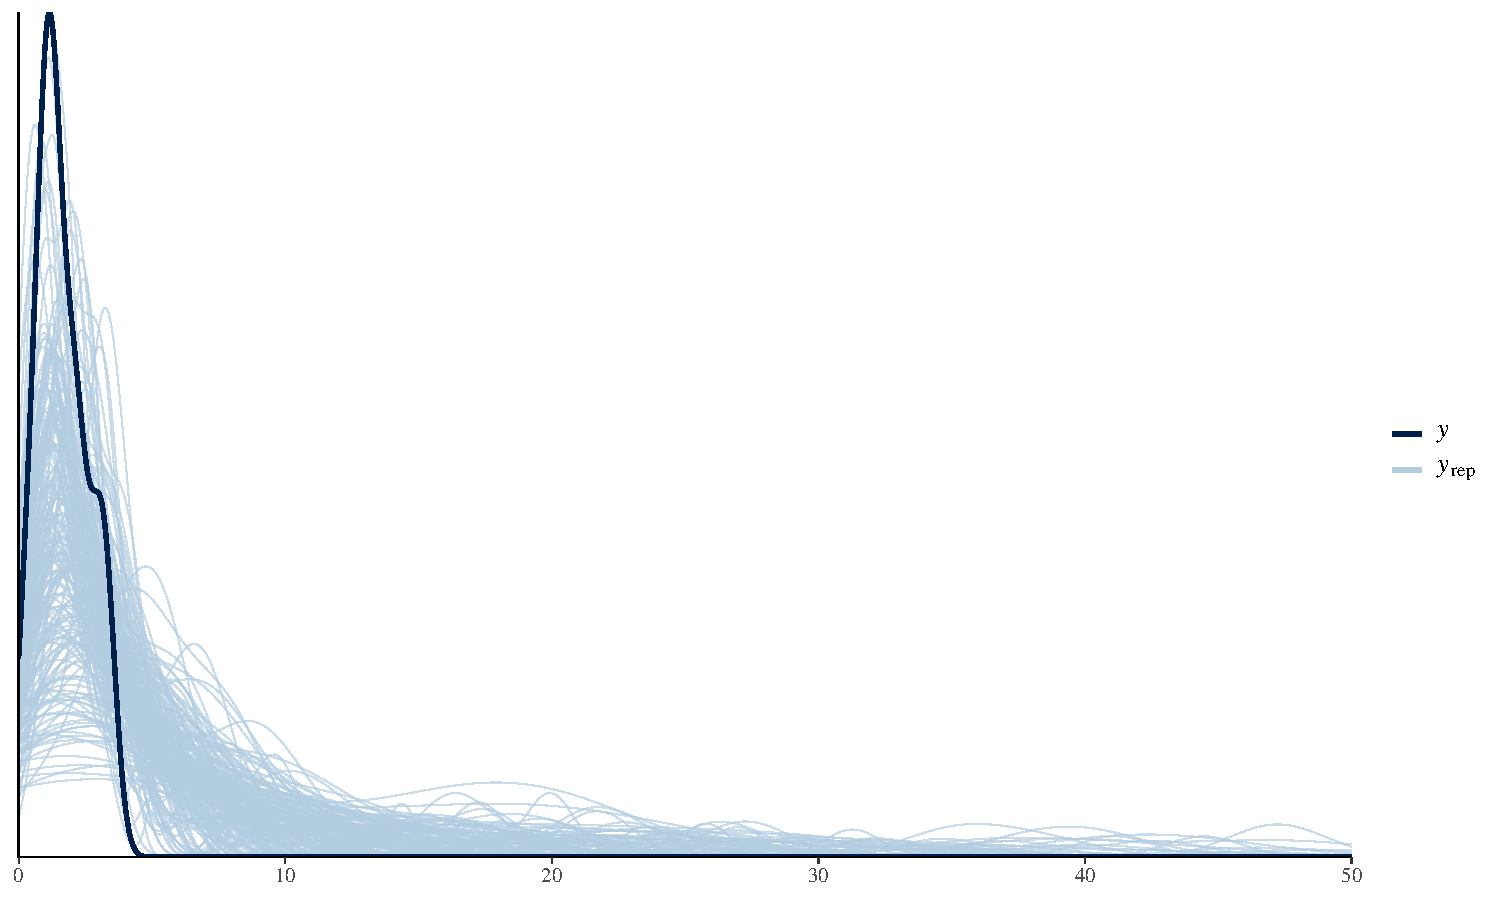
\includegraphics{DB_presentation_case_study_files/figure-beamer/unnamed-chunk-12-1.pdf}

\end{frame}

\begin{frame}{MCMC diagnostics: traceplot}

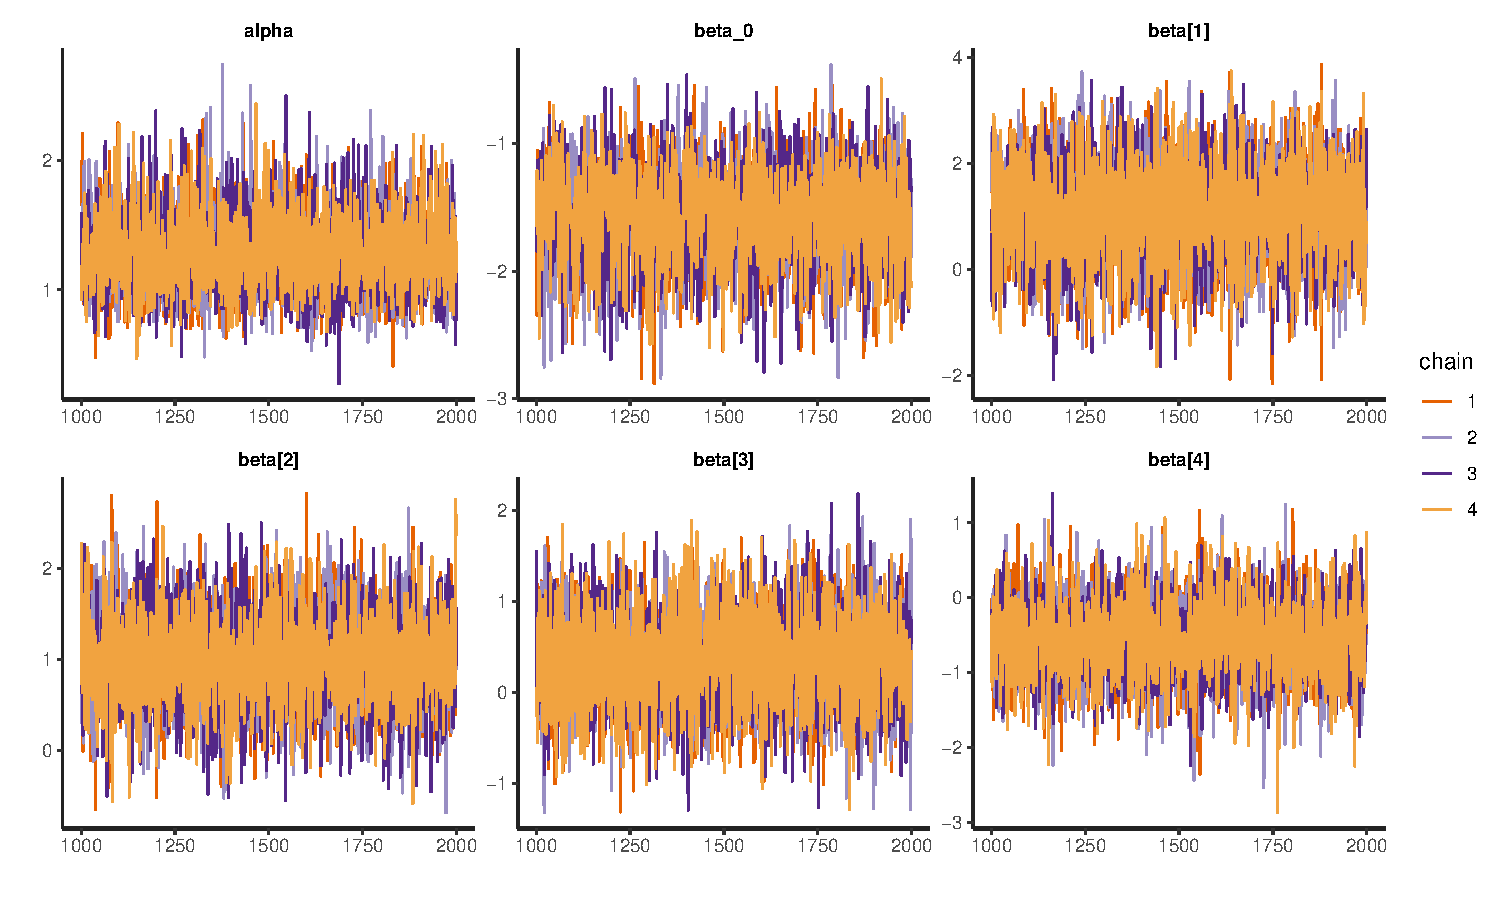
\includegraphics{DB_presentation_case_study_files/figure-beamer/unnamed-chunk-13-1.pdf}

\end{frame}

\begin{frame}{Posterior calibration (1)}

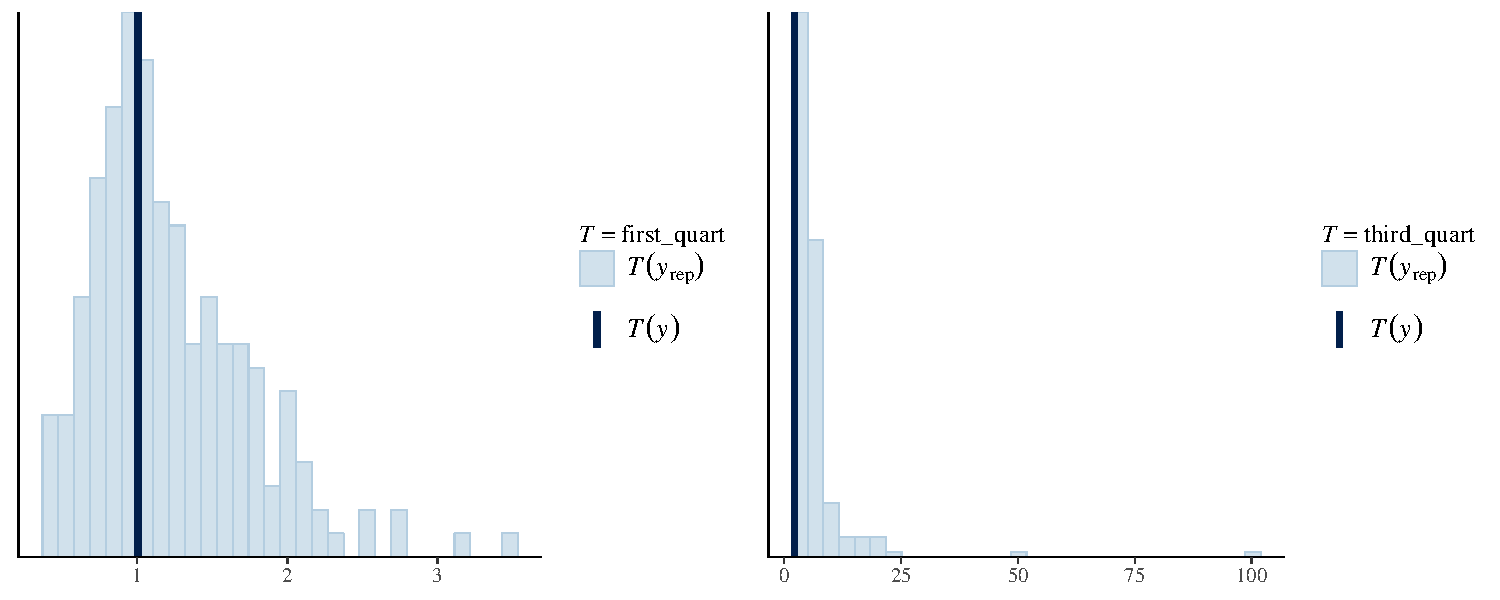
\includegraphics{DB_presentation_case_study_files/figure-beamer/unnamed-chunk-14-1.pdf}

\end{frame}

\begin{frame}{Posterior calibration (2)}

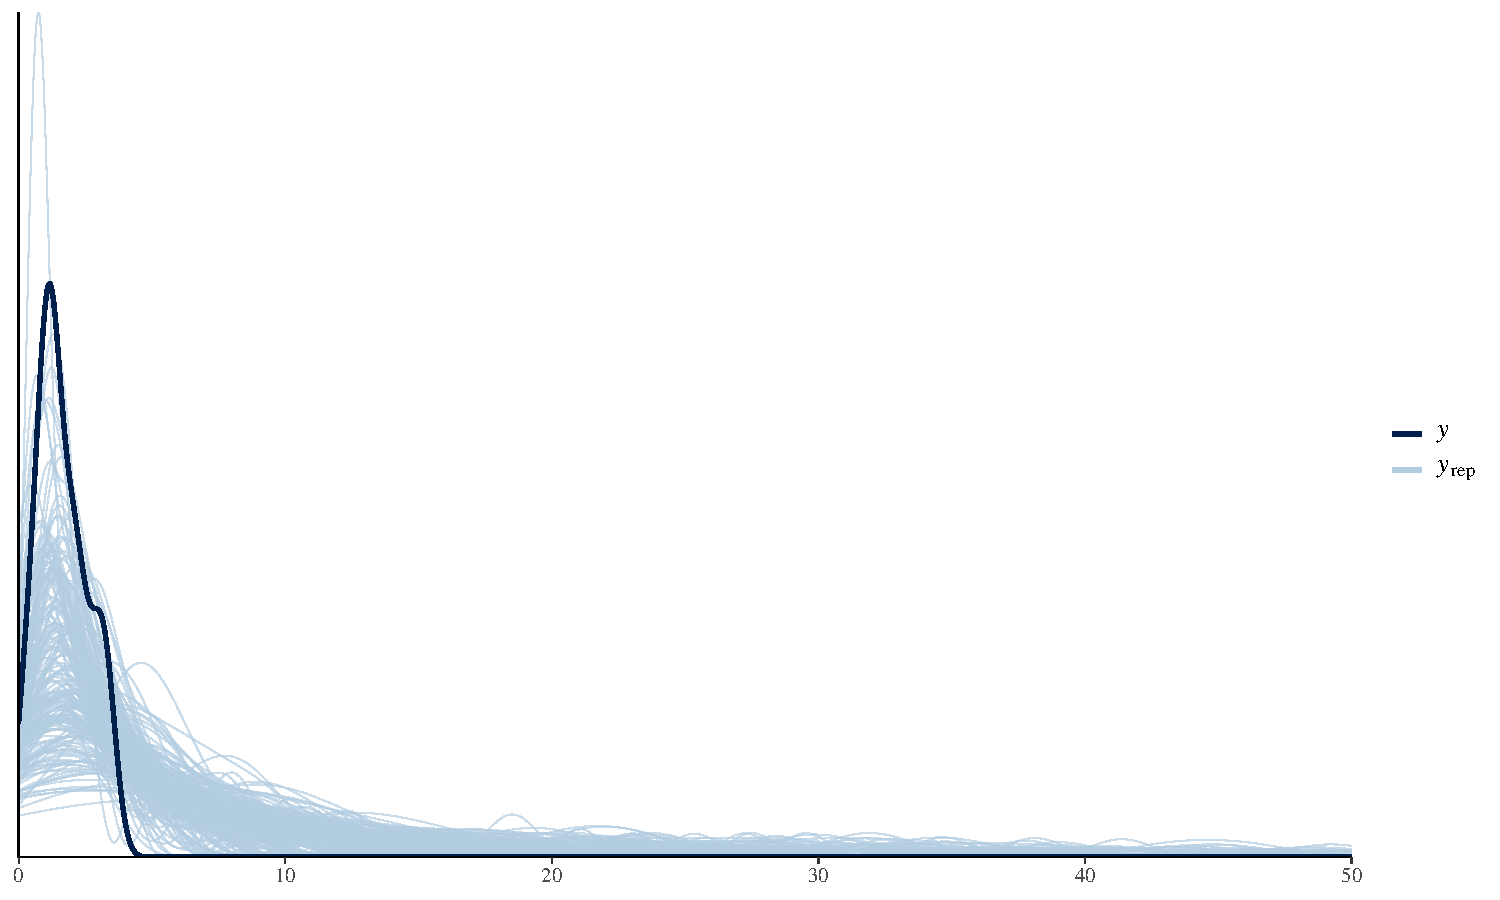
\includegraphics{DB_presentation_case_study_files/figure-beamer/unnamed-chunk-15-1.pdf}

\end{frame}

\begin{frame}{Posterior calibration (3)}

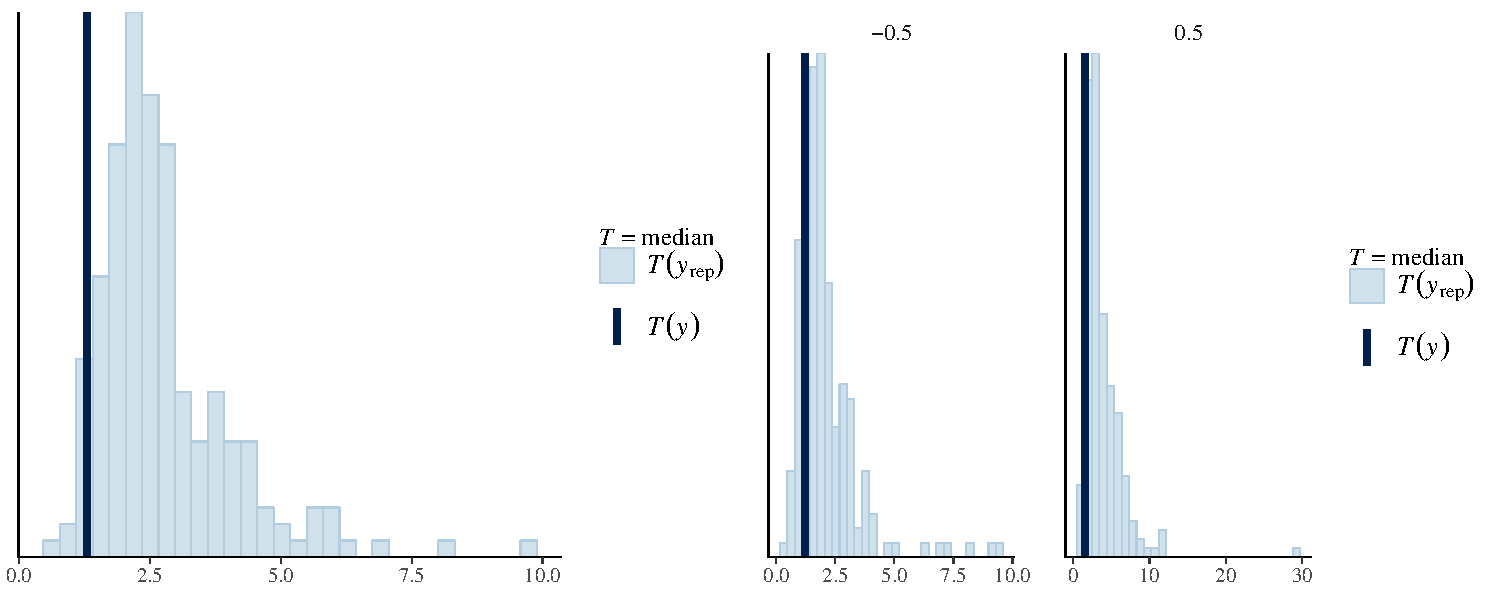
\includegraphics{DB_presentation_case_study_files/figure-beamer/unnamed-chunk-16-1.pdf}

\end{frame}

\begin{frame}{Revise the model}

\begin{itemize}
  \item{The model predicts greater follow-up times than those observed
        in the ovarian cancer data}
  \item{Weibull distribution may not be the best one to model 
        time-to-deaths of subjects with ovarian cancer}
  \item{Different family distributions can be considered, e.g.
        log-normal, gamma, ...}
\end{itemize}

\end{frame}

\begin{frame}{Log-normal (1)}

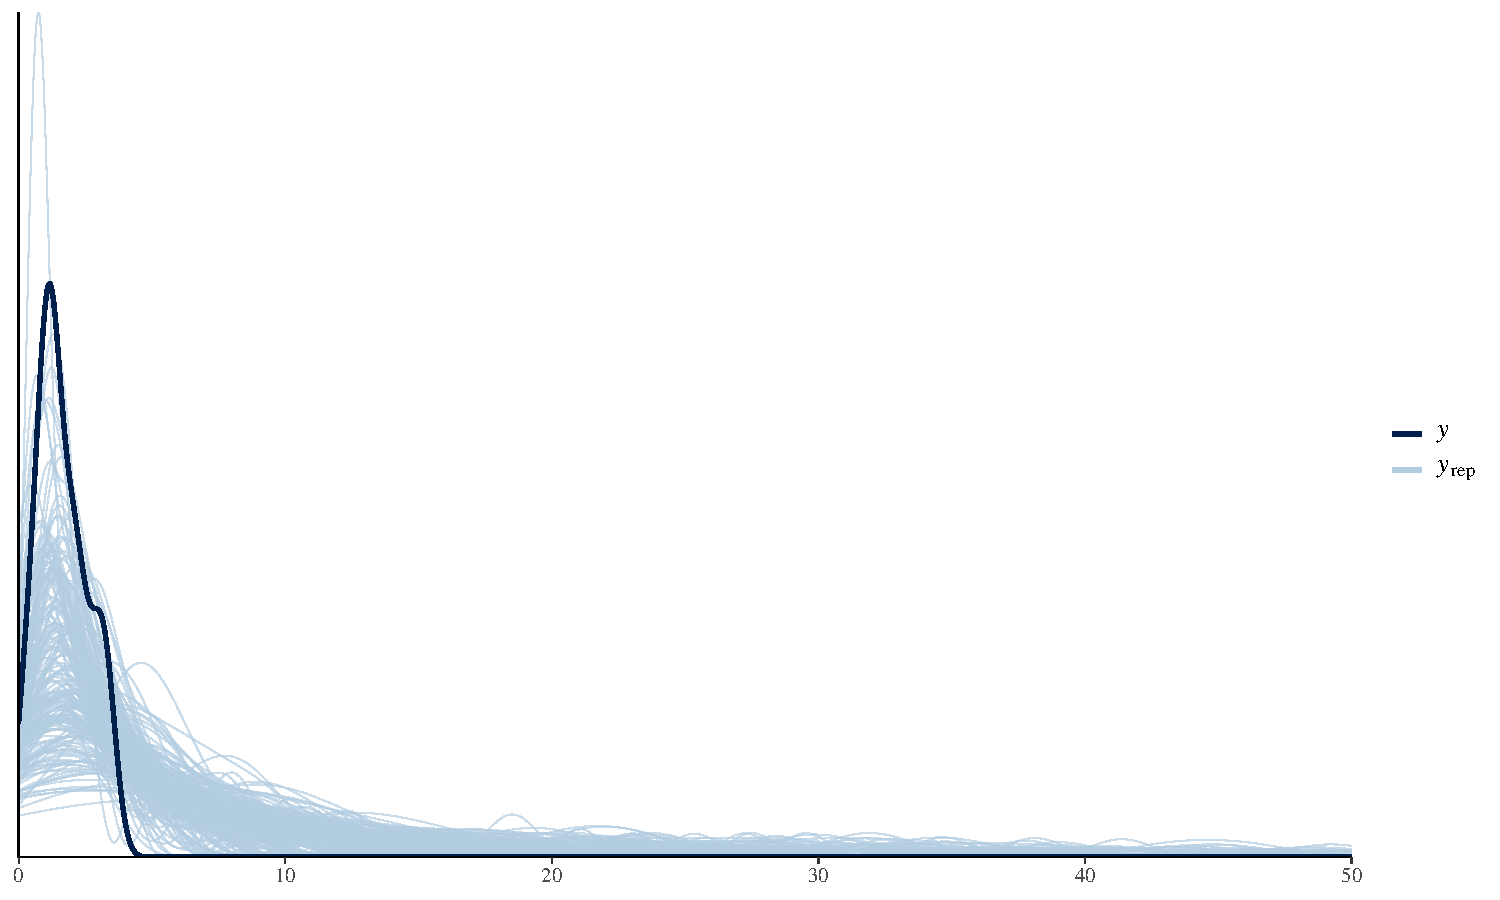
\includegraphics{DB_presentation_case_study_files/figure-beamer/unnamed-chunk-17-1.pdf}

\end{frame}

\begin{frame}{Log-normal (2)}

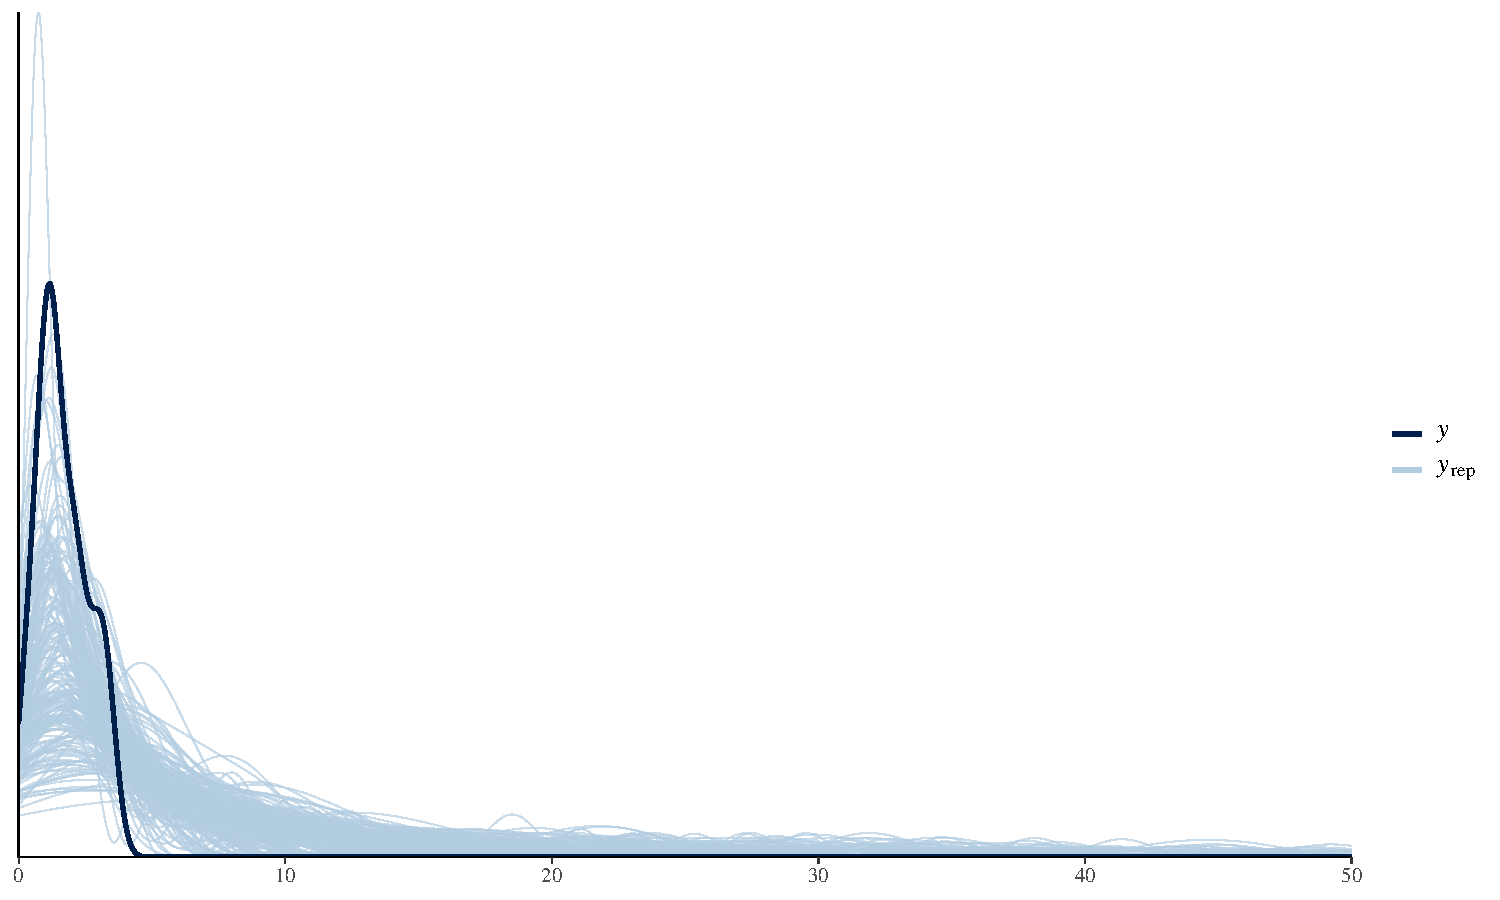
\includegraphics{DB_presentation_case_study_files/figure-beamer/unnamed-chunk-18-1.pdf}

\end{frame}

\begin{frame}{Log-normal (3)}

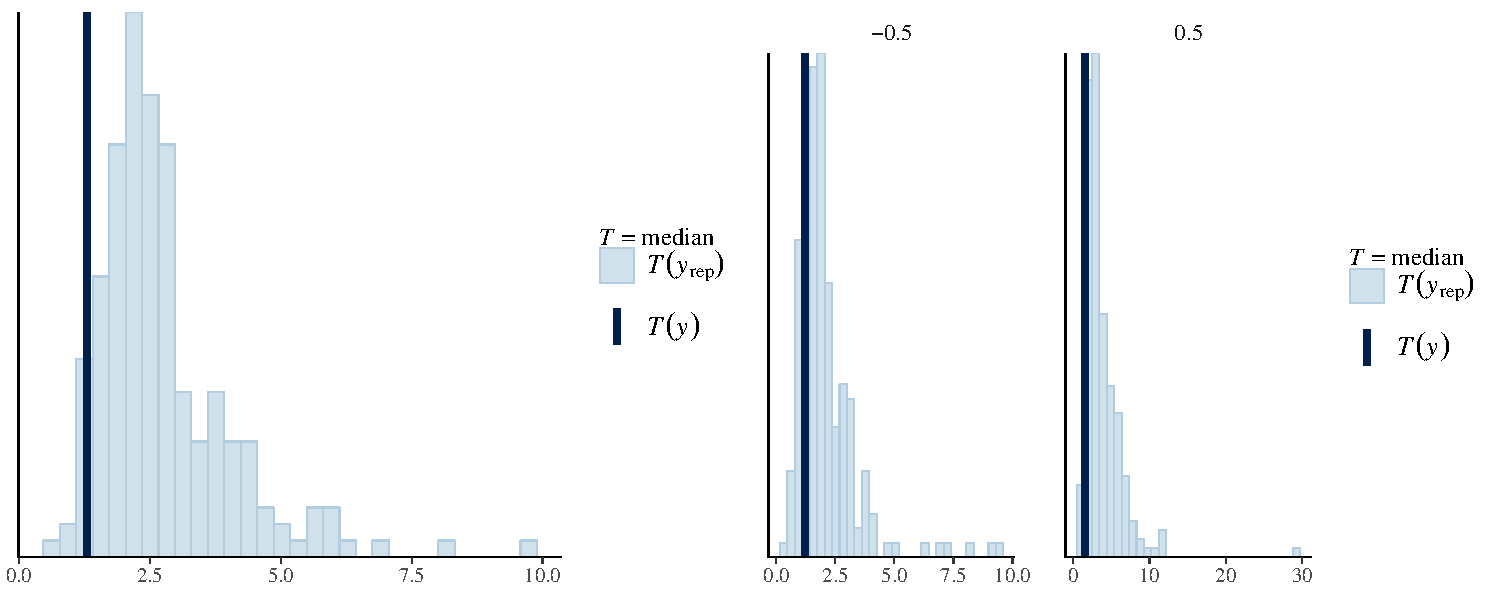
\includegraphics{DB_presentation_case_study_files/figure-beamer/unnamed-chunk-19-1.pdf}

\end{frame}

\begin{frame}{Gamma (1)}

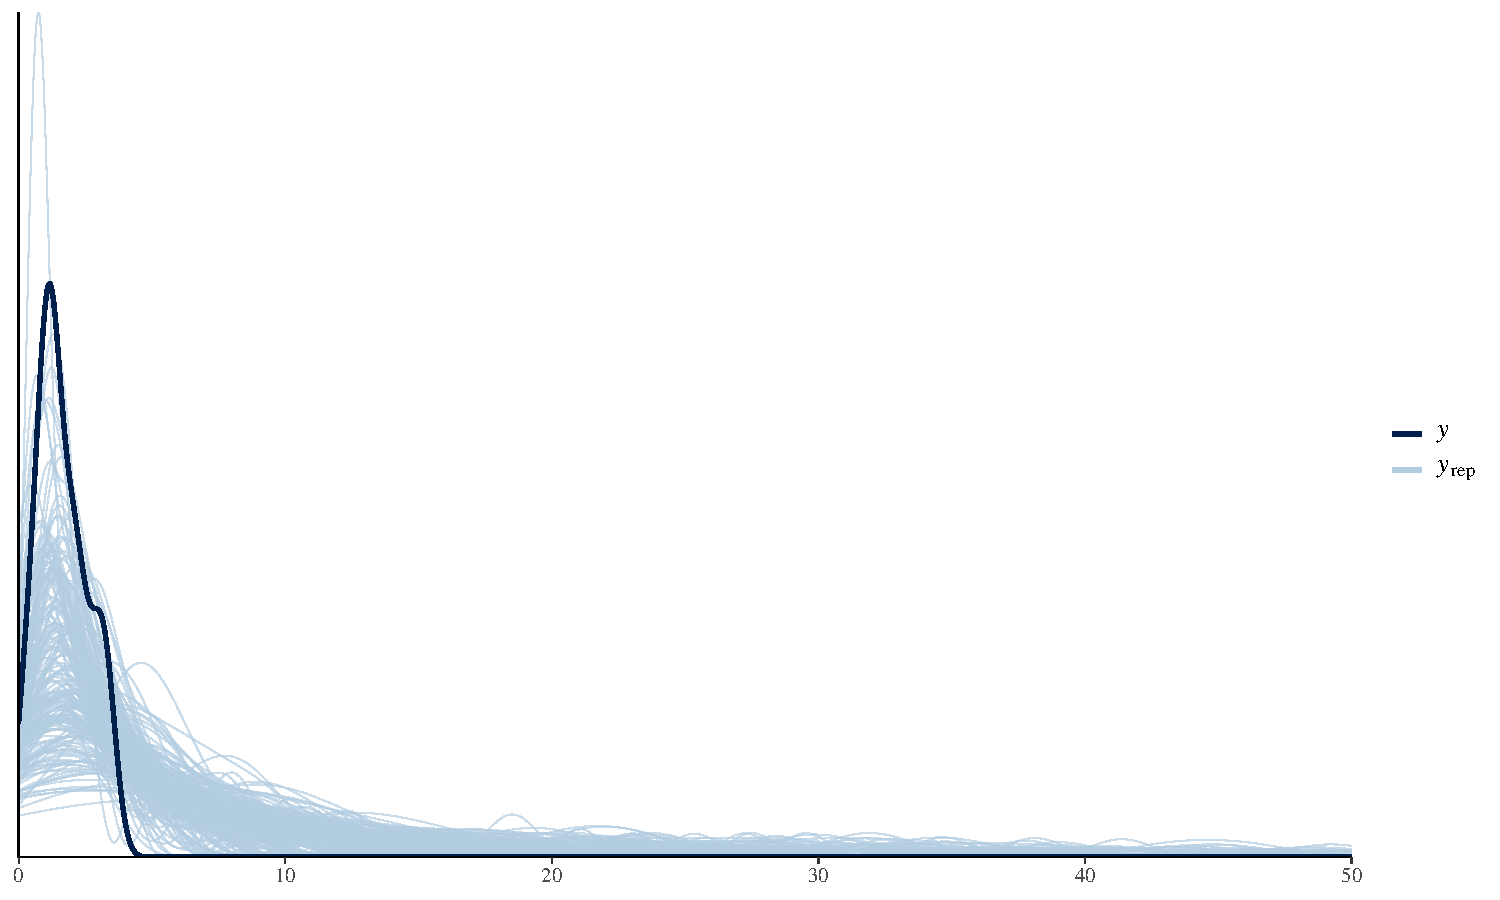
\includegraphics{DB_presentation_case_study_files/figure-beamer/unnamed-chunk-20-1.pdf}

\end{frame}

\begin{frame}{Gamma (2)}

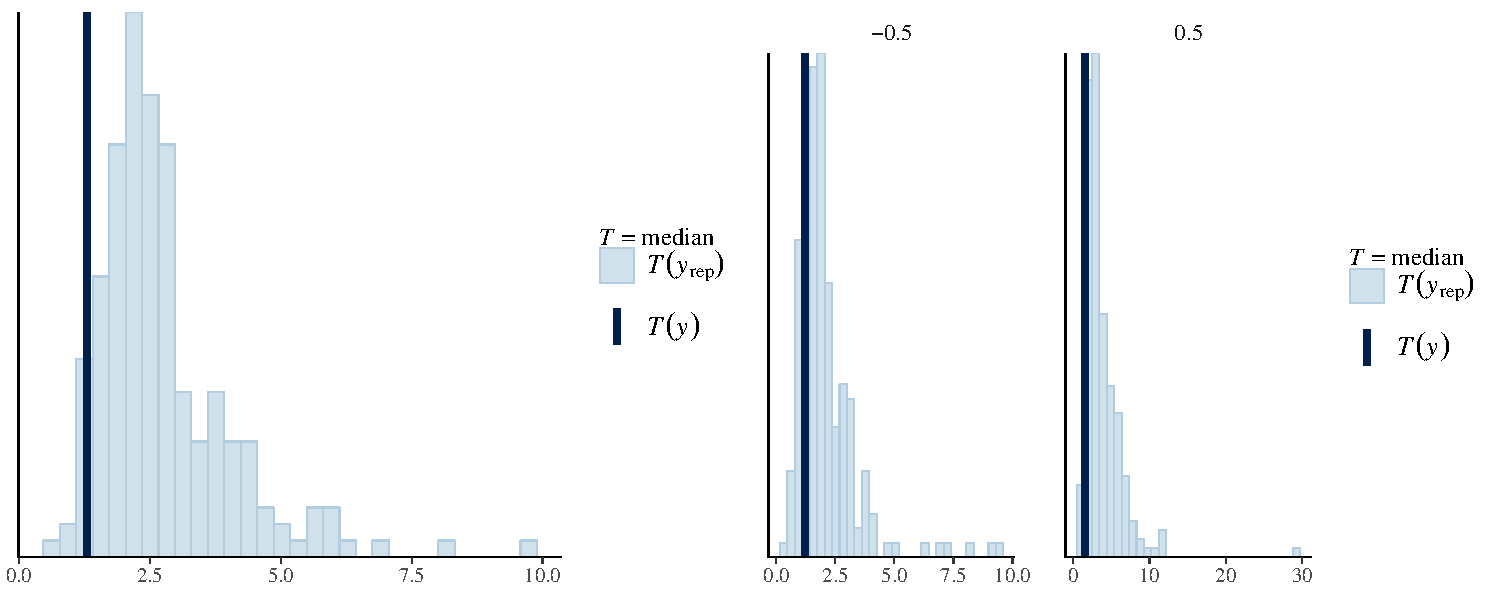
\includegraphics{DB_presentation_case_study_files/figure-beamer/unnamed-chunk-21-1.pdf}

\end{frame}

\begin{frame}{Gamma (3)}

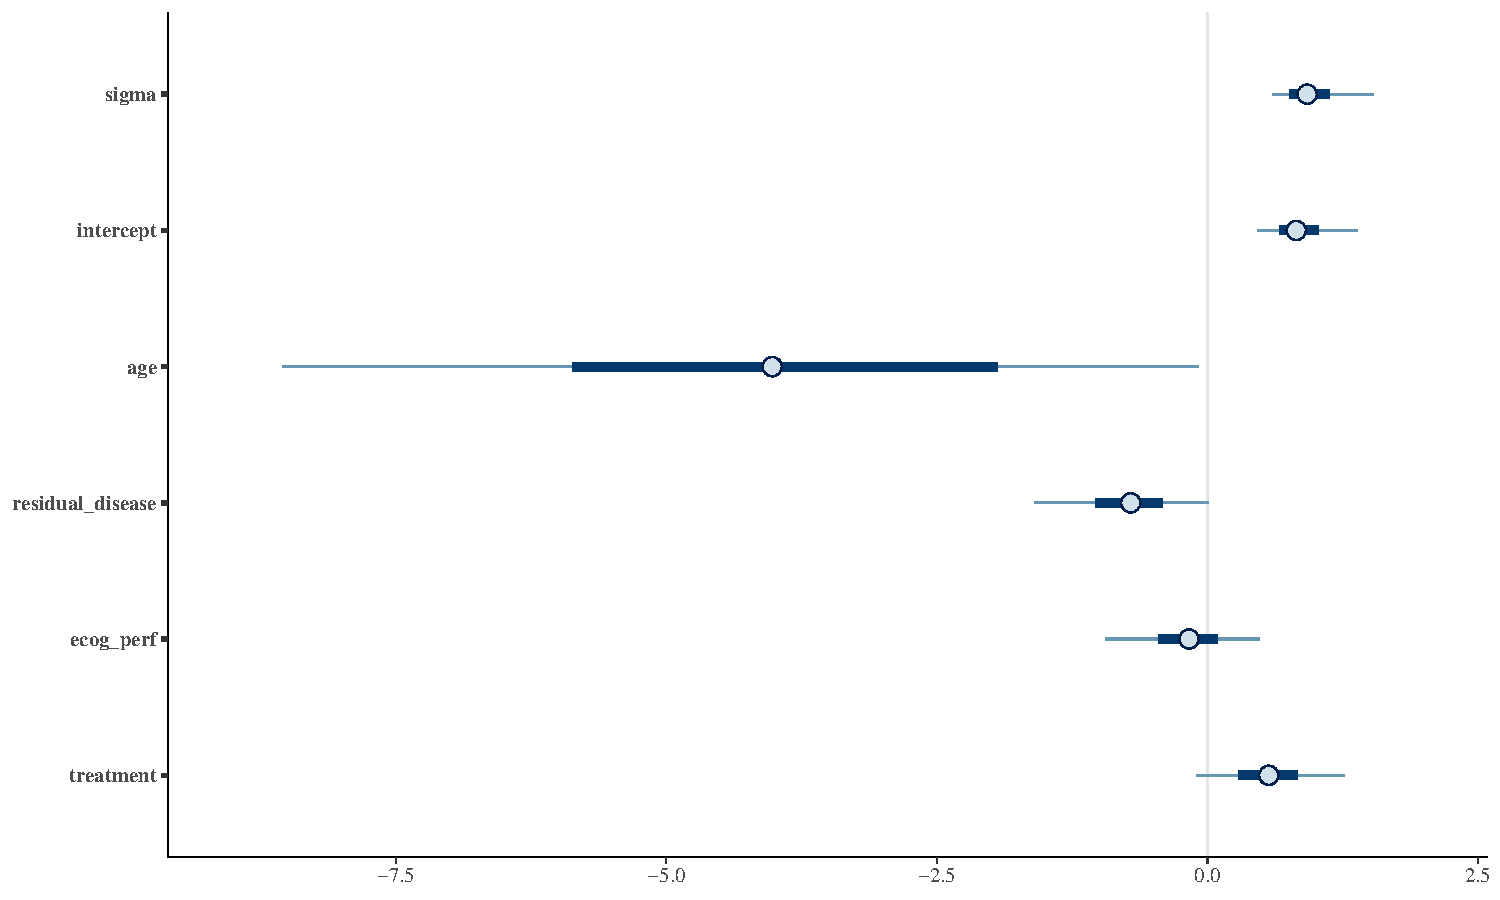
\includegraphics{DB_presentation_case_study_files/figure-beamer/unnamed-chunk-22-1.pdf}

\end{frame}

\begin{frame}{Compare the models (1)}

\begin{itemize}
\setlength\itemsep{1em}
  \item{Models can be compared by using leave-one-out cross-validation
        (LOO-CV)}
  \item{Expected log predictive density (ELPD) computed with LOO-CV
        can be used to evaluate which model has a better fit}
  \item{Predictive weights can be assigned to each model by using
        Stacking, Pseudo bayesian-model-averaging (Pseudo-BMA)}
  \item{Higher ELPD and predictive weights suggest better 
        predictive performances}
\end{itemize}

\end{frame}

\begin{frame}{Compare the models (2)}

\scriptsize

\begin{longtable}[]{@{}lrrr@{}}
\caption{Comparison of ELPD of the fitted models.}\tabularnewline
\toprule
model & elpd\_diff & elpd\_loo & se\_elpd\_loo\tabularnewline
\midrule
\endfirsthead
\toprule
model & elpd\_diff & elpd\_loo & se\_elpd\_loo\tabularnewline
\midrule
\endhead
lognormal & 0.00 & -23.95 & 3.13\tabularnewline
gamma & -1.28 & -25.23 & 3.27\tabularnewline
weibull & -4.02 & -27.97 & 3.40\tabularnewline
\bottomrule
\end{longtable}

\begin{longtable}[]{@{}lrrr@{}}
\caption{Model comparison with Stacking, Pseudo-BMA and Pseudo-BMA with
Bayesian Bootstrap.}\tabularnewline
\toprule
model & stacking & pseudo\_bma & pseudo\_bma\_bb\tabularnewline
\midrule
\endfirsthead
\toprule
model & stacking & pseudo\_bma & pseudo\_bma\_bb\tabularnewline
\midrule
\endhead
weibull & 0 & 0.014 & 0.047\tabularnewline
lognormal & 1 & 0.772 & 0.736\tabularnewline
gamma & 0 & 0.214 & 0.217\tabularnewline
\bottomrule
\end{longtable}

\end{frame}

\begin{frame}{Parameters of the model (1)}

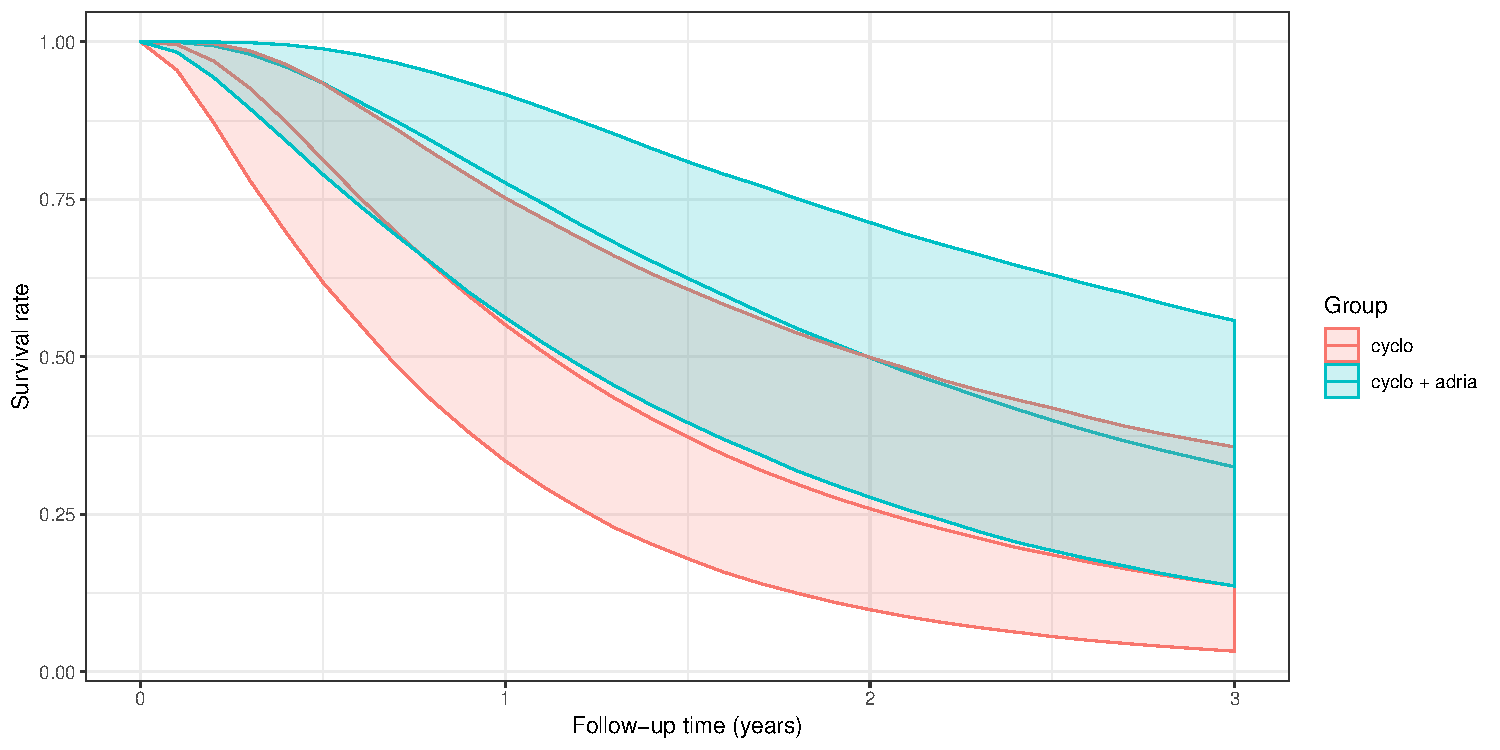
\includegraphics{DB_presentation_case_study_files/figure-beamer/unnamed-chunk-24-1.pdf}

\end{frame}

\begin{frame}{Parameters of the model (2)}

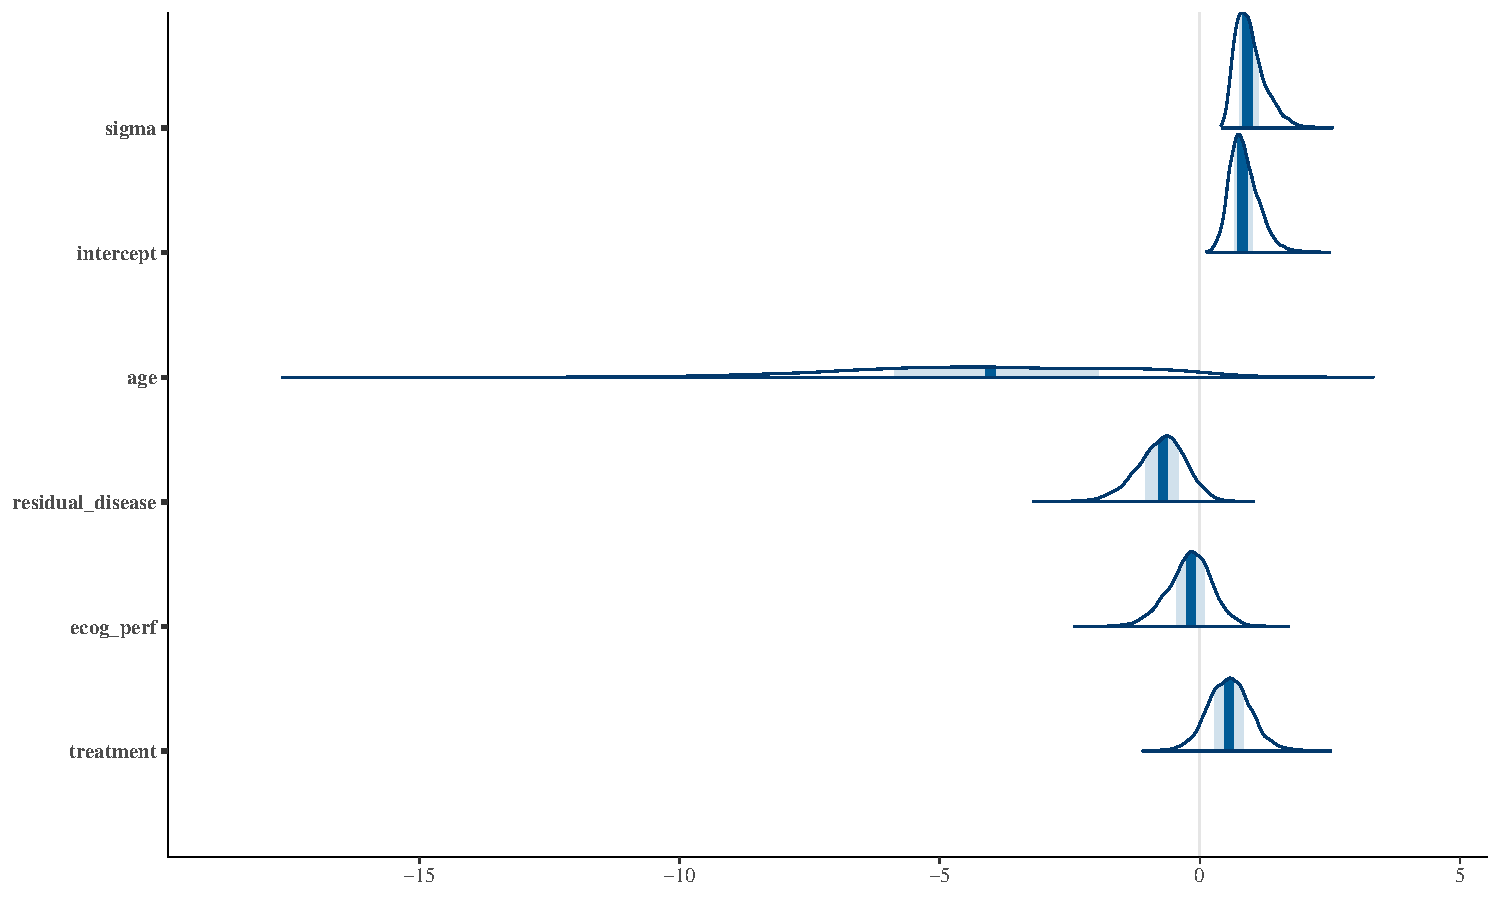
\includegraphics{DB_presentation_case_study_files/figure-beamer/unnamed-chunk-25-1.pdf}

\end{frame}

\begin{frame}{Posterior predictive survival curves}

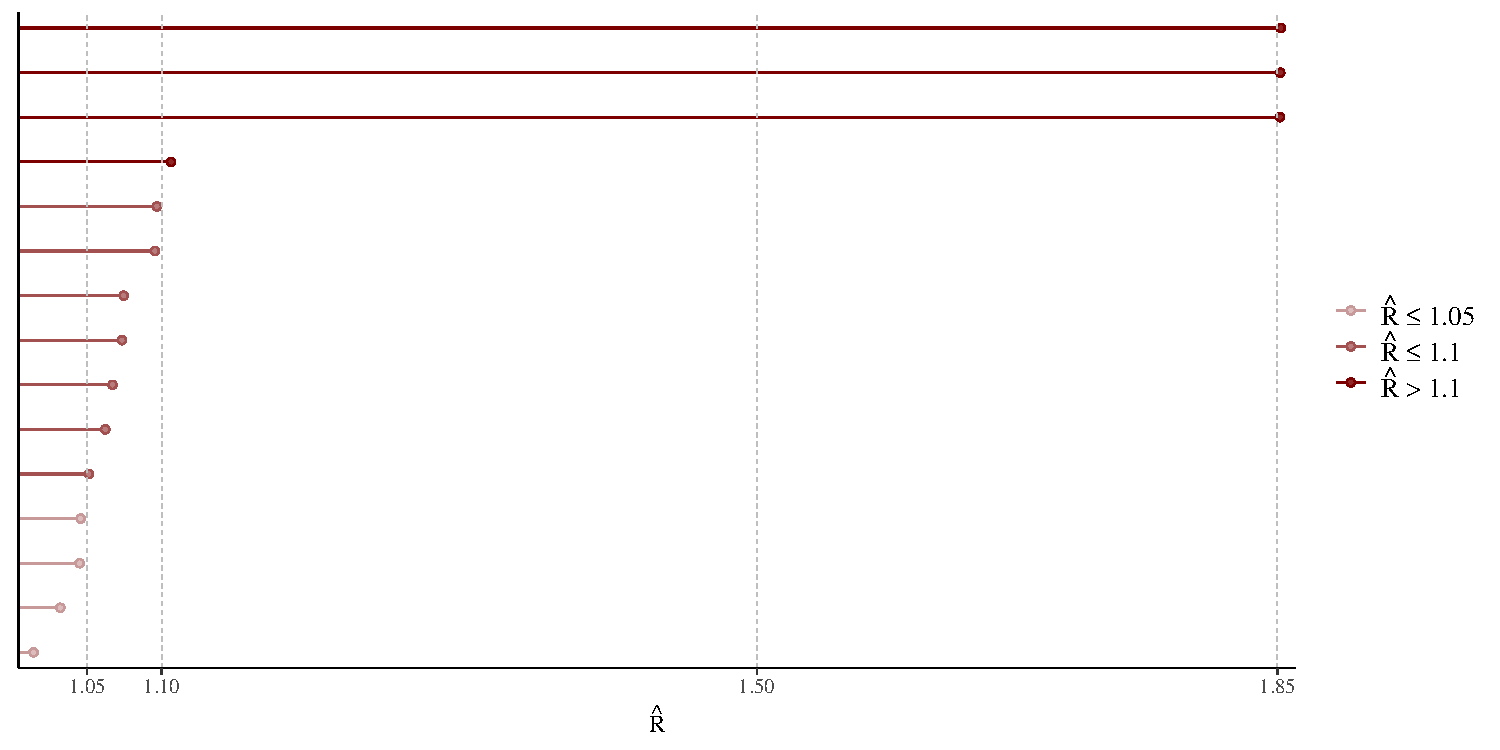
\includegraphics{DB_presentation_case_study_files/figure-beamer/unnamed-chunk-26-1.pdf}

\end{frame}

\section{Logistic Regression Case
Study}\label{logistic-regression-case-study}

\begin{frame}{Influenza vaccine case study}

\begin{itemize}
\item
  Hospitalized adults with acute respiratory disease tested for
  influenza with laboratory test (RT-PCR) (Talbot et al. 2013)
\item
  The aim of the study was to estimate vaccine effectiveness in reducing
  risk of influenza
\item
  Case-positive, control-negative study design
\item
  Low prevalence of influenza (\(\approx 10 \%\))
\end{itemize}

\end{frame}

\begin{frame}{The data}

\begin{itemize}
\item
  Data were simulated from the information provided by \emph{Chen et al.
  (2016)} (Chen et al., n.d.):
\item
  \(200\) subjects
\item
  \(19\) with positive influenza status and \(119\) with verified
  vaccination status
\item
  \(13\) confounders: race, home oxygen use, current smoking status,
  diabetes mellitus, asthma chronic obstructive pulmonary disease,
  chronic heart disease, immunosuppression, chronic liver or kidney
  disease, asplenia, and other type of disease
\end{itemize}

\end{frame}

\begin{frame}{The goal}

\begin{itemize}
\item
  With low number of cases and high number of covariates a standard
  logistic regression would overfit the data
\item
  In their study, \emph{Chen et al. (2016)} showed the benefits of
  penalizing maximum likelihood estimates (MLE) of all the terms in the
  model but the one related to the vaccination status
\item
  Control both for overfitting and bias in the exposure estimate
\item
  How can prior distributions help in such situations?
\end{itemize}

\end{frame}

\begin{frame}{Non-informative uniform priors}

\end{frame}

\begin{frame}{Non-informative uniform priors}

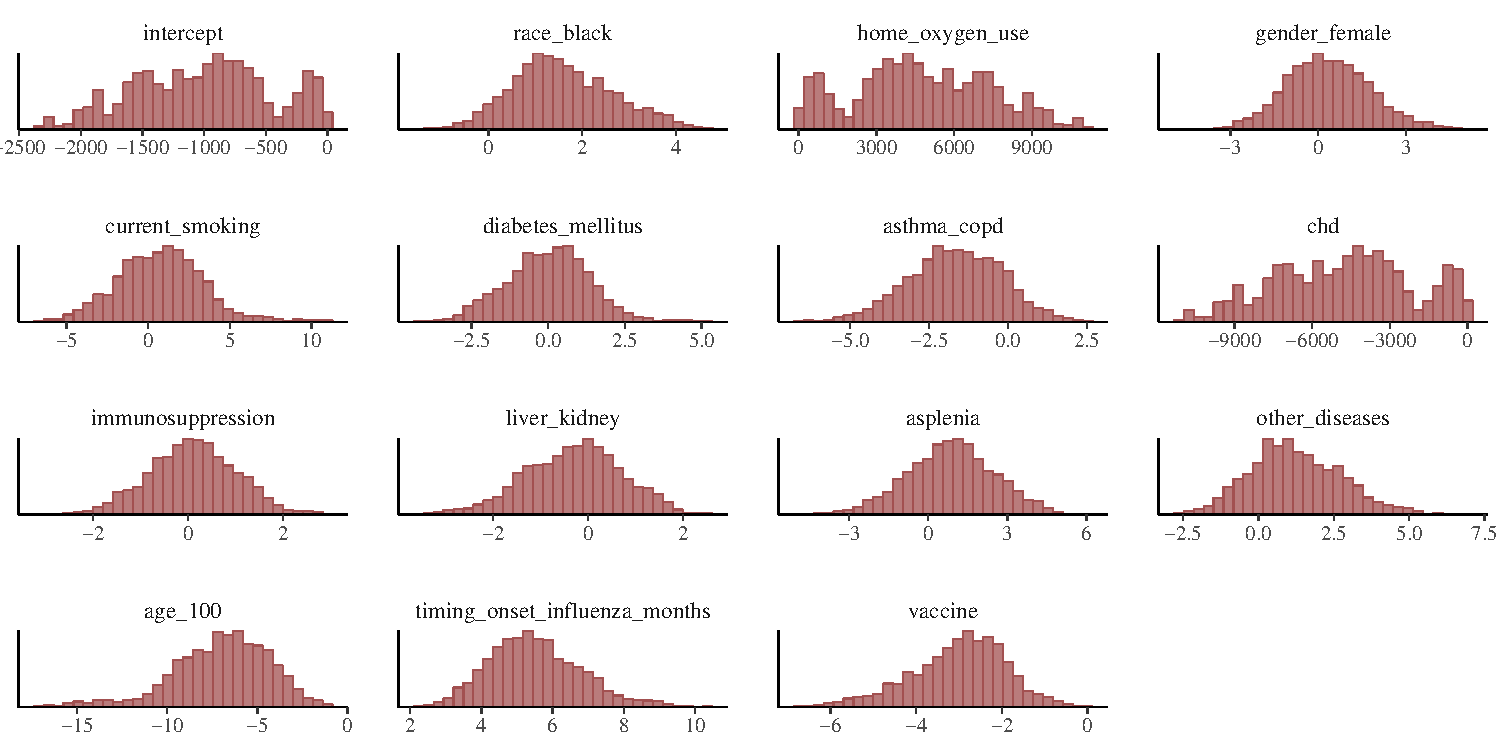
\includegraphics{DB_presentation_case_study_files/figure-beamer/unnamed-chunk-27-1.pdf}

\end{frame}

\begin{frame}{Non-informative uniform priors}

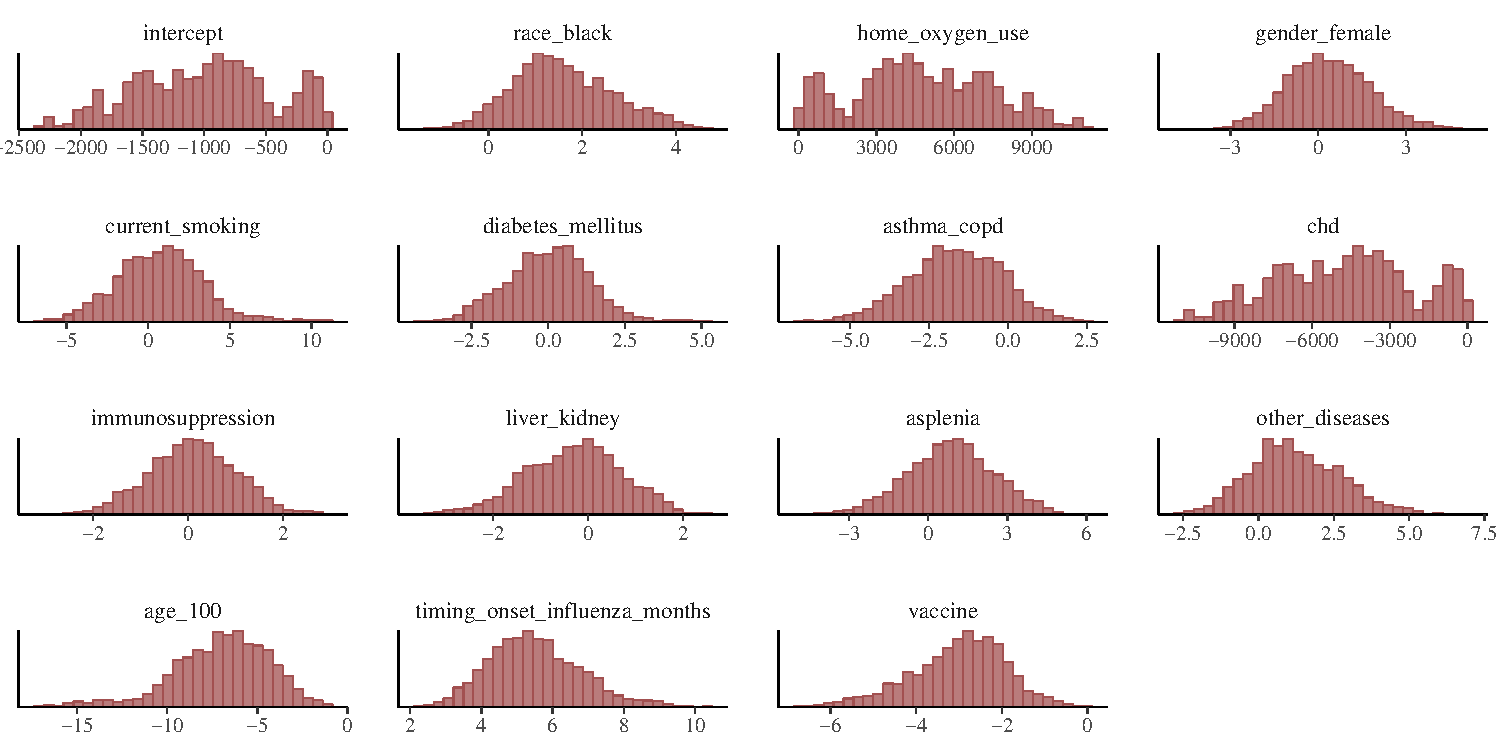
\includegraphics{DB_presentation_case_study_files/figure-beamer/unnamed-chunk-28-1.pdf}

\end{frame}

\begin{frame}{Non-informative uniform priors}

\begin{itemize}
\item
  Coefficients estimates are too extreme to be plausible
\item
  The algorithm did not perform a good sample of the posterior:

  \begin{itemize}
  \tightlist
  \item
    Many divergent transitions
  \item
    Low \(R_{hat}\) and \(ESS\) values
  \end{itemize}
\item
  The model likely overfitted the data
\item
  Priors that allow for less extreme values may help
\end{itemize}

\end{frame}

\begin{frame}{Vague priors: \(N \sim \left( 0, 100 \right)\)}

\end{frame}

\begin{frame}{Vague priors: \(N \sim \left( 0, 100 \right)\)}

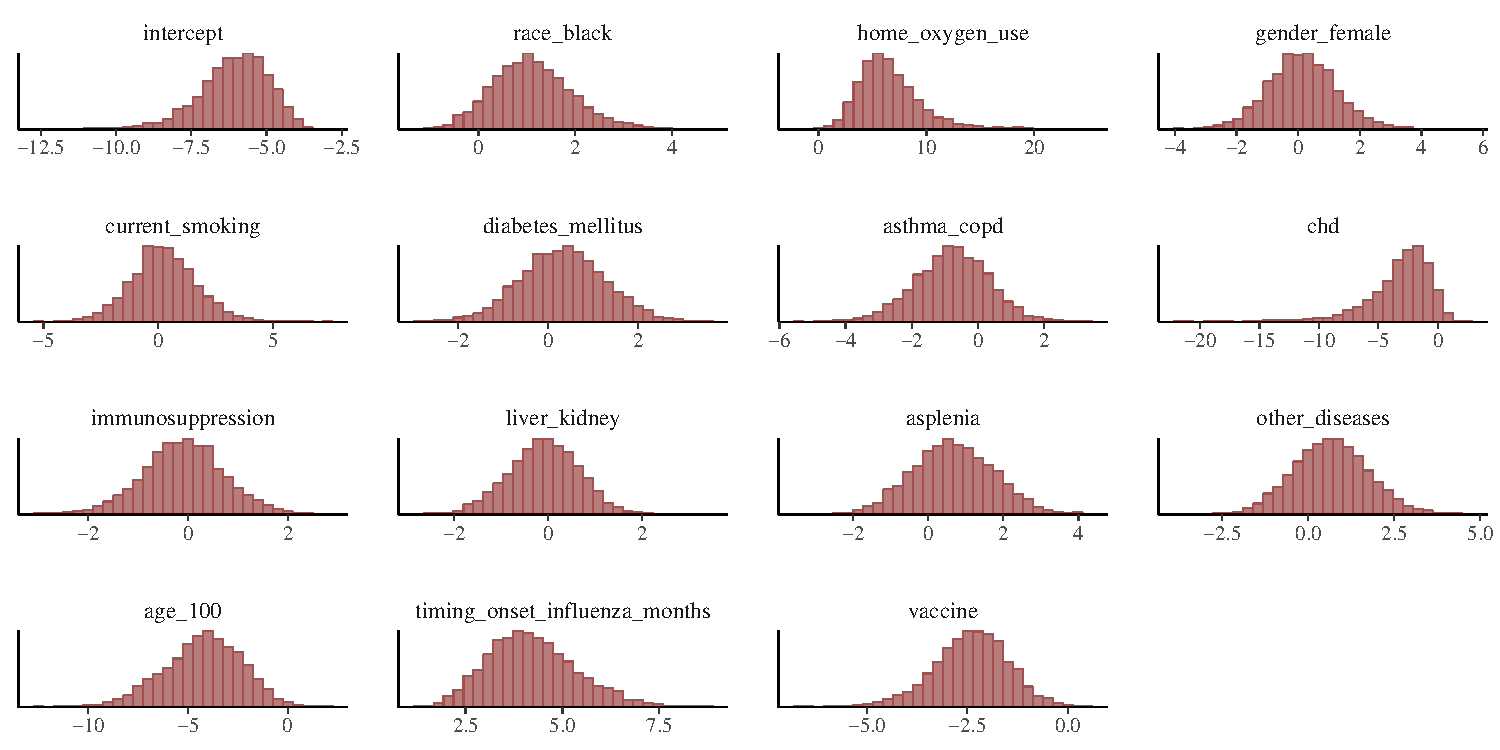
\includegraphics{DB_presentation_case_study_files/figure-beamer/unnamed-chunk-29-1.pdf}

\end{frame}

\begin{frame}{Vague priors: \(N \sim \left( 0, 100 \right)\)}

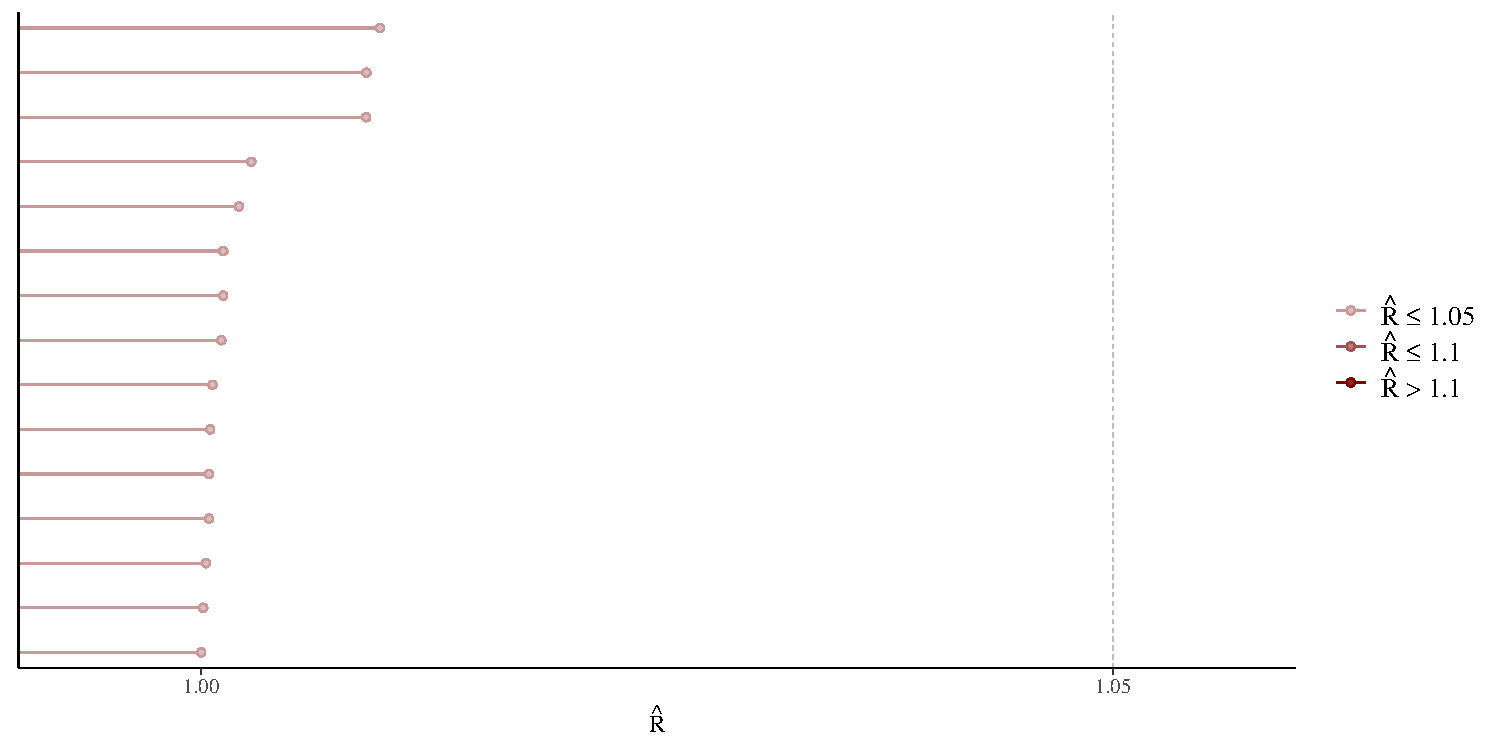
\includegraphics{DB_presentation_case_study_files/figure-beamer/unnamed-chunk-30-1.pdf}

\end{frame}

\begin{frame}{\(Cauchy \sim \left( 0, 2.5 \right)\)}

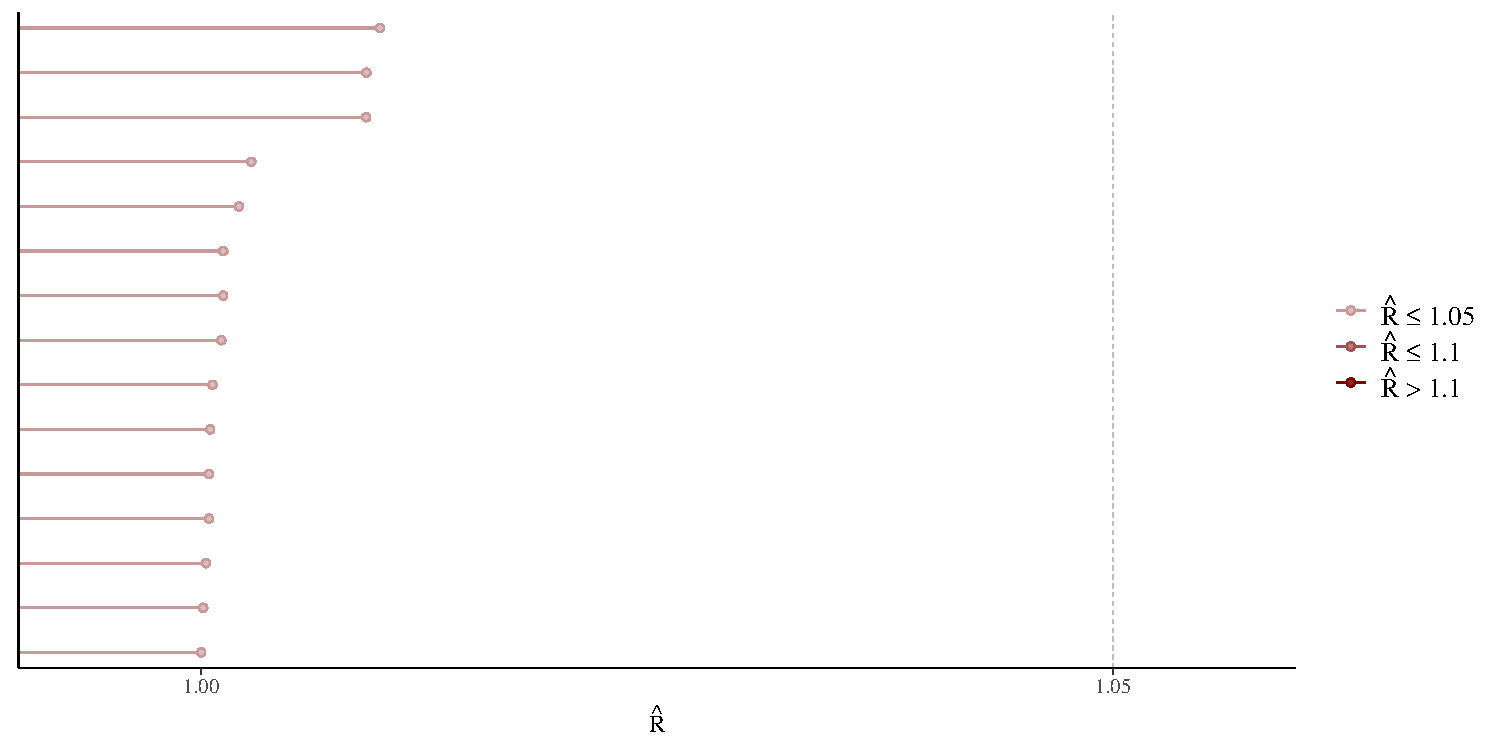
\includegraphics{DB_presentation_case_study_files/figure-beamer/unnamed-chunk-31-1.pdf}

\end{frame}

\begin{frame}{\(Cauchy \sim \left( 0, 2.5 \right)\)}

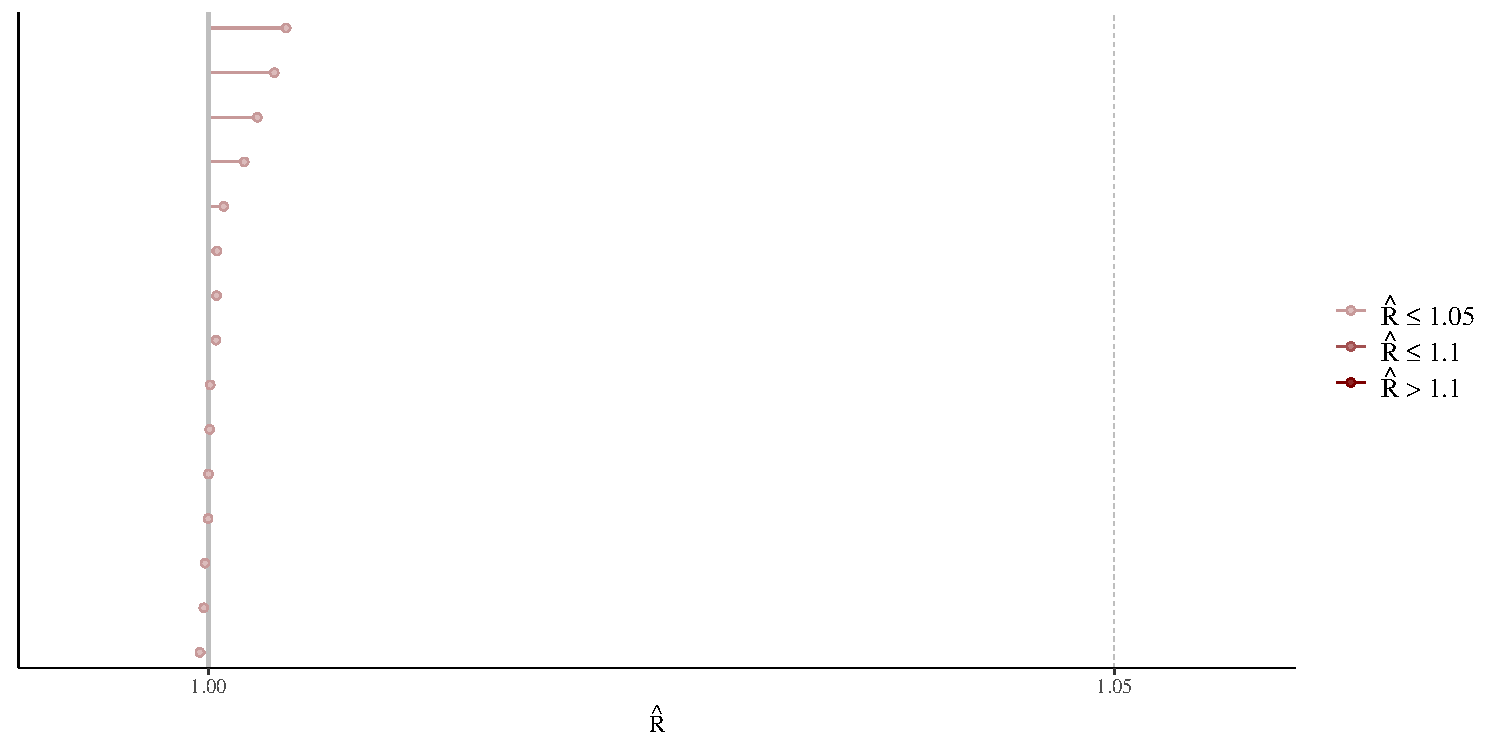
\includegraphics{DB_presentation_case_study_files/figure-beamer/unnamed-chunk-32-1.pdf}

\end{frame}

\begin{frame}{Weakly informative priors}

\begin{itemize}
\item
  \(Cauchy \sim \left( 0, 2.5 \right)\) improved the fit, but
  overfitting may be still present given the high values of coefficients
\item
  Weakly informative priors may help in such situations to regularize
  inference by shrinking regression coefficients to \(0\)
\item
  The idea is to give more probability to values near the \(0\) while
  giving at the same time some chances to higher values
\item
  If covariates are roughly on unit scale,
  \(t-student \sim \left(df, 0, 1 \right)\) with \(3 \leq df \leq 7\) is
  a reasonable choice for logistic regression models
\end{itemize}

\end{frame}

\begin{frame}{T-student priors: coefficients}

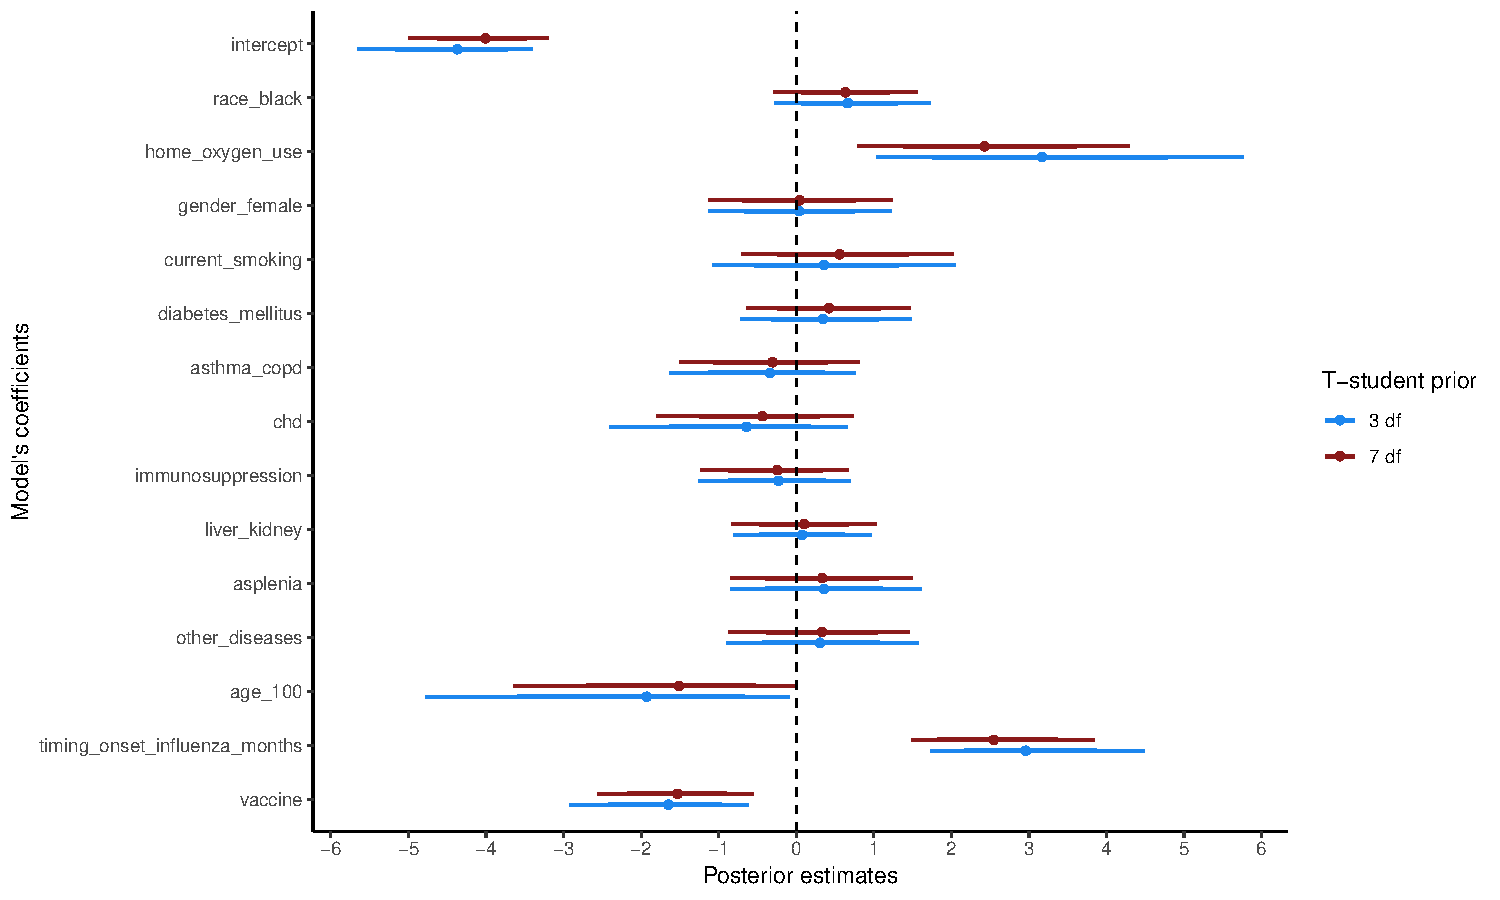
\includegraphics{DB_presentation_case_study_files/figure-beamer/unnamed-chunk-33-1.pdf}

\end{frame}

\begin{frame}{T-student priors: posterior checks (1)}

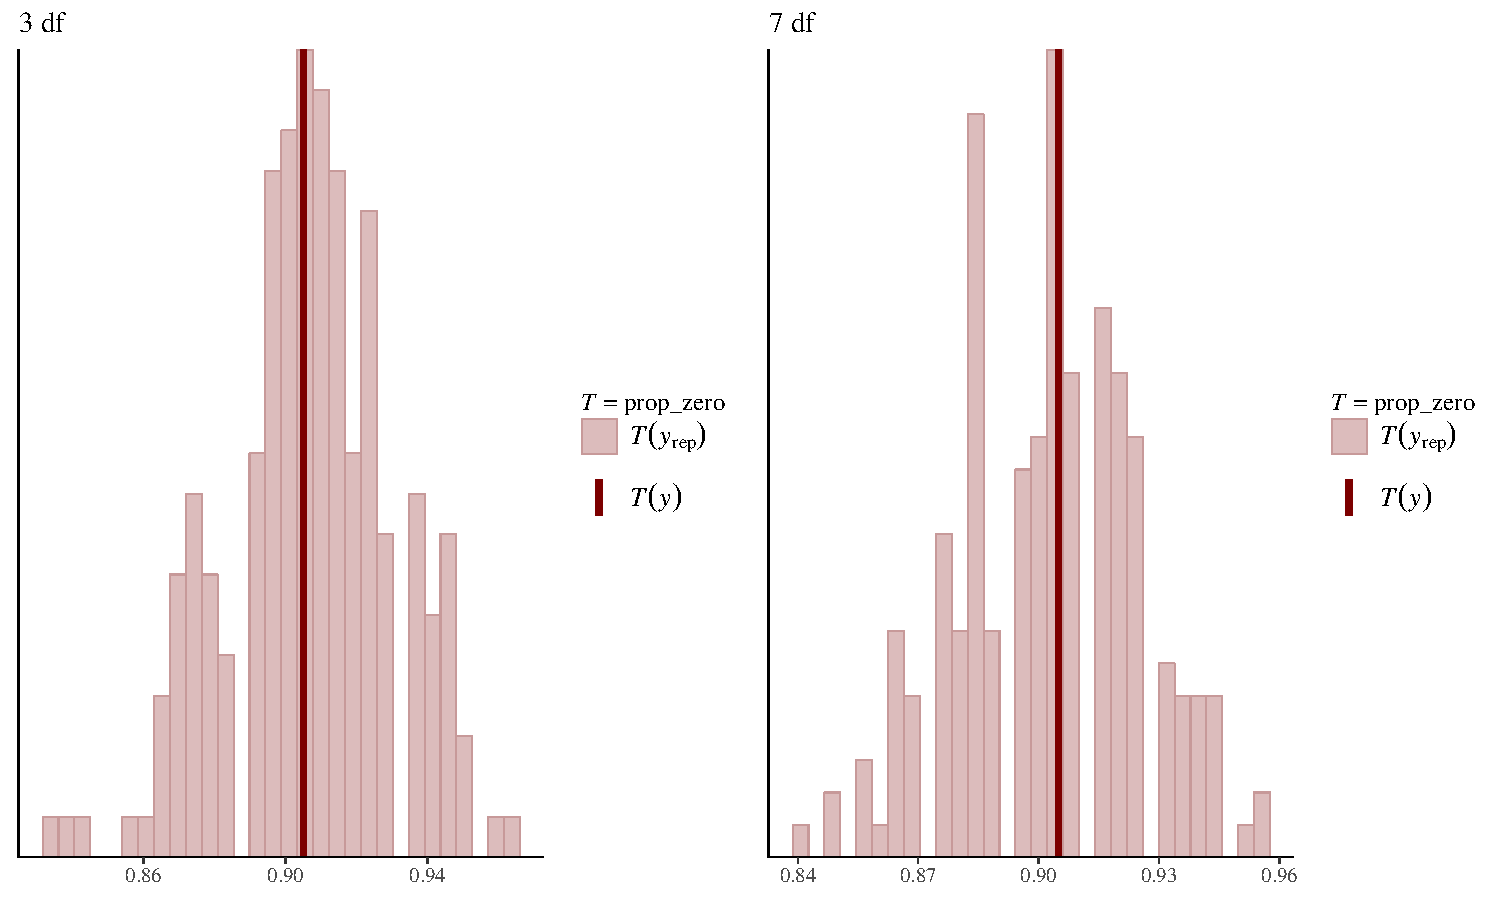
\includegraphics{DB_presentation_case_study_files/figure-beamer/unnamed-chunk-34-1.pdf}

\end{frame}

\begin{frame}{T-student priors: posterior checks (2)}

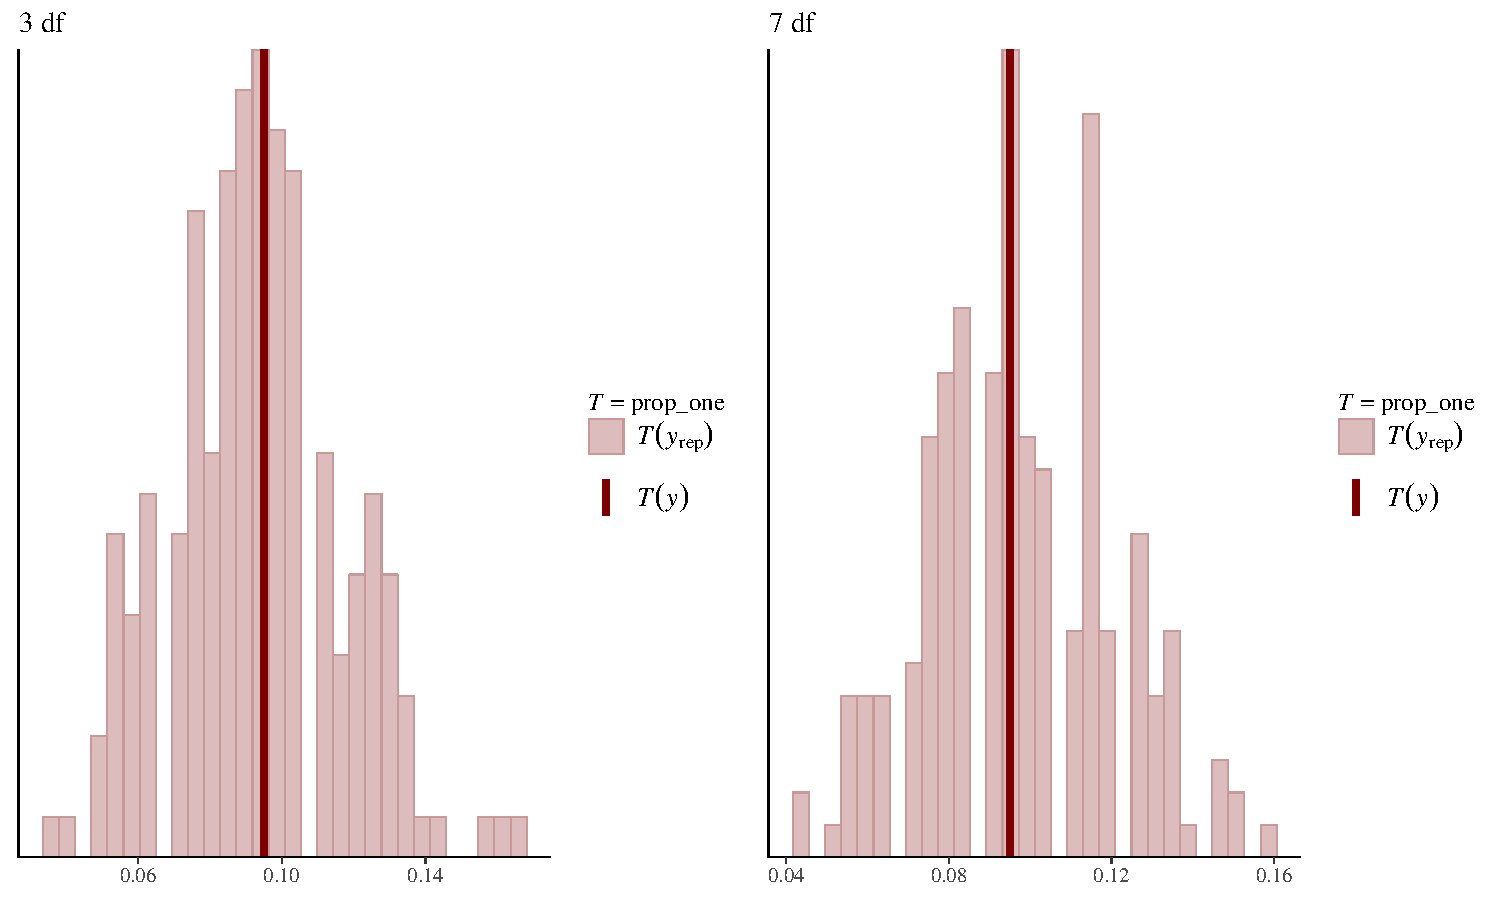
\includegraphics{DB_presentation_case_study_files/figure-beamer/unnamed-chunk-35-1.pdf}

\end{frame}

\begin{frame}{T-student priors: model comparison and averaging}

\begin{longtable}[]{@{}lrrr@{}}
\caption{Model comparison with Stacking, Pseudo-BMA and Pseudo-BMA with
Bayesian Bootstrap.}\tabularnewline
\toprule
model & stacking & pseudo\_bma & pseudo\_bma\_bb\tabularnewline
\midrule
\endfirsthead
\toprule
model & stacking & pseudo\_bma & pseudo\_bma\_bb\tabularnewline
\midrule
\endhead
student\_t\_3 & 0.579 & 0.333 & 0.307\tabularnewline
student\_t\_7 & 0.001 & 0.179 & 0.202\tabularnewline
student\_t\_3\_unp & 0.419 & 0.300 & 0.320\tabularnewline
student\_t\_7\_unp & 0.000 & 0.188 & 0.171\tabularnewline
\bottomrule
\end{longtable}

\end{frame}

\begin{frame}{Vaccine effectiveness}

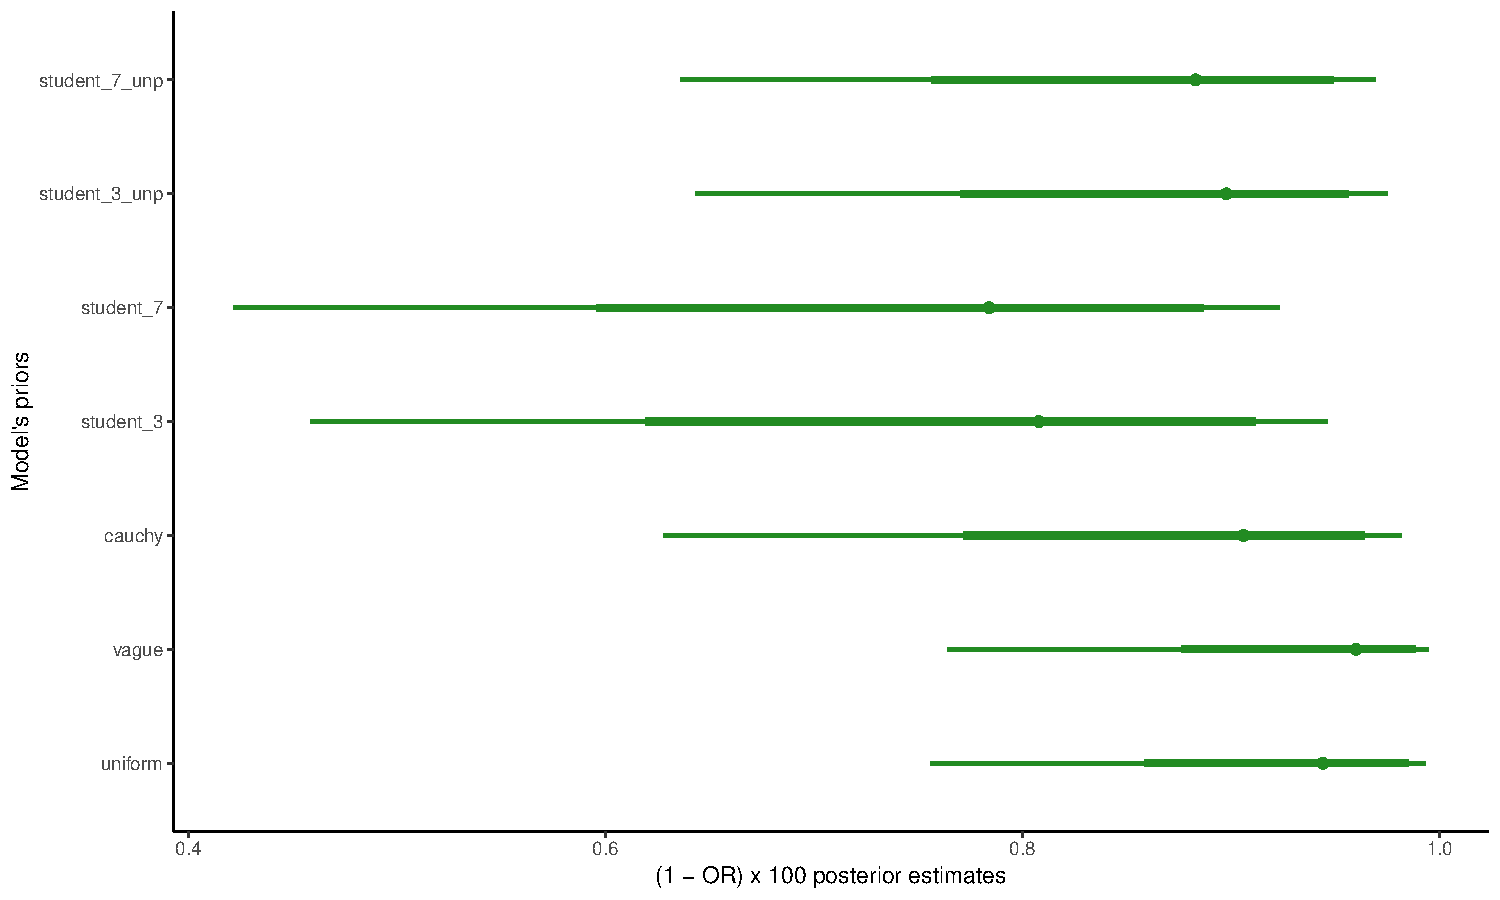
\includegraphics{DB_presentation_case_study_files/figure-beamer/unnamed-chunk-37-1.pdf}

\end{frame}

\begin{frame}{Additional information}

\begin{itemize}
\item
  Stan's website at \url{http://mc-stan.org/}. Here you can find the
  reference manual, videos, tutorials, case studies and so on
\item
  Here's a list of R packages that interface with Stan:

  \begin{itemize}
  \tightlist
  \item
    \textbf{rstan}
  \item
    \textbf{bayesplot}
  \item
    \textbf{loo}
  \item
    \textbf{brms}
  \item
    \textbf{rstanarm}
  \item
    \textbf{trialr}
  \item
    \textbf{RBesT}
  \item
    \textbf{survHE}
  \end{itemize}
\item
  The slides of the presentation, the R and Stan codes used for the case
  studies are at \url{https://github.com/danielebottigliengo/IBIG_2018}
\end{itemize}

\end{frame}

\begin{frame}{References}

\footnotesize

\hypertarget{refs}{}
\hypertarget{ref-chen_2016}{}
Chen, Qingxia, Hui Nian, Yuwei Zhu, H. Keipp Talbot, Marie R. Griffin,
and Frank E. Harrell. n.d. ``Too Many Covariates and Too Few Cases? -- A
Comparative Study.'' \emph{Statistics in Medicine} 35 (25): 4546--58.
doi:\href{https://doi.org/10.1002/sim.7021}{10.1002/sim.7021}.

\hypertarget{ref-edmonson_1979}{}
Edmonson, J. H., T. R. Fleming, D. G. Decker, G. D. Malkasian, E. O.
Jorgensen, J. A. Jefferies, M. J. Webb, and L. K. Kvols. 1979.
``Different Chemotherapeutic Sensitivities and Host Factors Affecting
Prognosis in Advanced Ovarian Carcinoma Versus Minimal Residual
Disease.'' \emph{Cancer Treatment Reports} 63 (2): 241--47.

\hypertarget{ref-talbot_2013}{}
Talbot, H. Keipp, Yuwei Zhu, Qingxia Chen, John V. Williams, Mark G.
Thompson, and Marie R. Griffin. 2013. ``Effectiveness of Influenza
Vaccine for Preventing Laboratory-Confirmed Influenza Hospitalizations
in Adults, 2011--2012 Influenza Season.'' \emph{Clinical Infectious
Diseases} 56 (12): 1774--7.
doi:\href{https://doi.org/10.1093/cid/cit124}{10.1093/cid/cit124}.

\end{frame}

\end{document}
